\documentclass[12pt]{report}
\usepackage[utf8]{inputenc}
\usepackage{graphicx}
\usepackage[a4paper,width=150mm,top=25mm,bottom=25mm]{geometry}
\usepackage{lipsum}
\usepackage{fancyhdr}

% Plain Title to be used later
% \title{An Empirical Analysis of Architectural Design Records}
% \author{Nikolaos Katsios}
% \date{Athens University of Economics and Business \\ \today}

\begin{document}

\begin{titlepage}
    \begin{center}
        \vspace*{1cm}
            
        \Huge
        \textbf{An Empirical Analysis of Architectural Design Records}
            
        \vspace{0.5cm}

        
\includegraphics[scale=0.5]{figures/athens_university_logo.png}
            
        \vspace{1.5cm}
            
        \textbf{Nikolaos Katsios}
            
        \vspace{0.8cm}
        
        \Large
        Athens University of Economics and Business \\
        Department of Management Science and Technology\\
        Date: 1/7/2024\\

        \Large
        Supervisor: Diomidis Spinellis
    \end{center}
\end{titlepage}

% \maketitle

% TODO: Enrich near the end
\begin{abstract}
    This thesis aims to explore and analyze architectural design records (ADRs) to understand their importance in documenting and guiding architectural decisions in software development projects. Through empirical analysis, this work seeks to uncover patterns, practices, and the impact of ADRs on project success.
\end{abstract}

\newpage
\tableofcontents
\listoffigures
\newpage

\chapter{Introduction}
    Software architecture has become an increasingly complex and multidimensional topic in the past years that gathers the interest and inspiration from various fields of study. When designing systems, various design decisions are made by architects that capture the functionality of the ever-increasingly intertwined components. By recognizing design decisions as first-class entities that address functional and non-functional requirements, software architecture is divided into many sub-tasks with logical continuity that may or may not depend on each other \cite{Arch+DesignDescisions}. This process, produces system knowledge also known as Architectural Knowledge (AK).
    However, without proper documentation, this knowledge often evaporates increasing the cost of maintenance and creating uncertainty and other adverse effects for all relevant system stakeholders. To combat this problem and provide information retention,  Architectural Design Records (ADRs) and relevant artifacts are employed as a strategic method to systematically document crucial decisions, capturing not only the outcome but also the rationale behind each decision. In the following chapters, a general overview of AK will be presented followed by ways to capture it using industry-validated tools and formats. Then, leveraging an enriched ADR dataset derived from a systematic mining software repositories (MSR) study, a set of questions will be proposed and answered to shed light on the trends and practices regarding architectural management using a plethora of analysis methodologies. Since ADRs are a highly practical topic, we will also observe how they are being used by practitioners to facilitate knowledge management via various mechanisms.

    % Overview of sections and why they were chosen
    The remainder of the study is structured as follows. Section 2 presents background concepts about architectural decision making and architectural knowledge management, providing context on the process of software architecture based on a literature review. Section 3 goes into detail about Architectural Decision Records (ADRs), including their definition, role, usage, types, tool support, and practical applications with the aim to comprehend how they can fit in the architecture life cycle and the benefits they provide. Section 4 explains the research methodology employed to propose research questions, gather and analyze the dataset of ADRs to uncover topics and trends. Section 5 further describes the ADR dataset and extraction process, including data collection, cleaning enrichment and quality. Section 6 presents the ADR dataset analysis, explaining the analysis methods and discussing the results to the research questions. Finally, Section 7 addresses the conclusions derived from the analysis and proposes sustainability practices for ADRs along with future research directions.

\chapter{Architectural Decision Making and Architectural Knowledge}
    \section{Architectural Decision Making}
        In their pursuit to meet functional and non functional requirements, software architects implicitly or explicitly make design decisions about the software architecture of a system. While research efforts in the past focused mainly on the view of software architecture as components and their connectors \cite{software_arch_in_practice_book}, the paradigm has shifted towards recognising those design decisions as first class entities.\cite{first-class-Arch-decisions}. This approach is considered to provide a better overview of the system's properties, as all decisions have profound impact on the system itself and its evolution can be traced more easily by serializing them into a "decision chain".

        The process of making an architectural decision, typically involves solving a problem by satisfying specific requirements, in a given context, by considering various alternatives and weighing their pros and cons to navigate through the solution space and finally reach a consensus on how to proceed on the implementation. A decision rationale can also be provided to justify the end result. These decisions can be made solely by a singe architect, a group of architects or, in more social approaches, a team of engineers and developers. The decision can determine a specific technology to be used \cite{developer-study-arch-decisions}or set standards for the whole system such as architectural patterns. For example, a technology-specific architectural decision may refer to the type of relational database to be used in a software project. The alternatives may include a MySQL database and a Microsoft SQL Server database. In the end maybe the MySQL database is used due to its open-source nature and lack of licensing requirements. A pattern decision may be related to the use of the model, view, controller (MVC) pattern in a web application. This defines the core of the system architecture and all subsequent decisions will depend on that view. 

        When finalizing architectural decisions, architects often omit considering certain aspects of the problem. First, rarely are architectural decisions standalone entities, and if one is solidified, it will most likely affect previous decisions and dependencies, making some of them obsolete. In addition, since the sum of decisions comprise the final architecture, architects often fail to consider how a decision can be reversed in the event of integration failure. Finally, the knowledge gained from considering different decisions is not a part of the system unless it has been documented. [cite here]

    \section{Architectural Knowledge}
        Architectural Knowledge (AK) is a multidisciplinary topic that is difficult to define. 
        An understanding from the reviewed literature \cite{architectural_knowledge_definitions} indicates that architectural knowledge includes not only the architectural design itself but also the design decisions, assumptions, context, and other factors that collectively explain why a particular solution is the way it is. This is in line with the decision making process discussed in the previous section. This knowledge spans the problem domain (defining what issues need to be addressed), through decision-making processes (how issues are to be addressed), to the solution domain (what has been implemented to address these issues) and is built up from many past collective decisions that are context specific (related to a specific system in question), also known as \textit{Application-specific knowledge} or domain specific (related to software architecture in the broad sense) also known as\textit{ Application-generic knowledge} \cite{Patterns+ArchDecisions}. This is why architects, often rely on intuition to derive the solution to an architectural problem. \cite{Patterns+ArchDecisions, archtitect_survey}.

        It is therefore evident that AK plays an important role in the whole software development life-cycle. It helps in laying a framework that defines how software components interact and integrate, which is crucial for ensuring system scalability, performance, and reliability. It encompasses the system's evolution so it can later be presented to all relevant stakeholders, and accurately calculate the cost of development and maintenance. It is also clear that AK should be widely shared rather than confined to silos or the expertise of specific architects. Given that AK consists of individual design decisions, these can be reusable and adaptable to various scenarios, thus saving both cost and effort. This cross-entity sharing however is only possible if AK is properly documented and managed.
        
    \section{Problems of software architecture and Architectural knowledge management}
    - see arch as design decicions
    - ARCHITECTURAL KNOWLEDGE SHARING (AKS)APPROACHES: A SURVEY RESEARCH
    \section{Mental models and Decision making}
        Role of experience and structured approaches.
    \section{Importance of Capturing AK}
        Importance of capturing AK for continuity and governance.
    \section{Overview of Tools, Evolution and Capabilities}
        Overview of traditional and modern tools for capturing AK.
        Evolution, capabilities, and comparison of these tools.

\chapter{Architectural Decision Records (ADRs)}
    \section{Definition, Role and Use}
        An emerging way to capture architectural design decisions (ADDs) and prevent knowledge vaporization are Architectural Decision Records(ADRs). ADRs are lightweight text 
        artifacts that capture the rationale behind ADDs by outlining some of the basic structure of such decisions\cite{MarkdownADRs}. Their simplistic nature allows them to be stored alongside other software artifacts such as source code in software repositories, internal company wikis and regular documentation \cite{DOCUMENTING_ARCHITECTURE_DECISIONS}. They can also be put under version control systems like Git in order to preserve their modification history as the requirements of the system in question change but they are mostly viewed as an append-only log\cite{microsoftArchitectureDecision} and thus, they are immutable. This means that if the need to revisit an existing architecture arises, there is a need to create an entirely new ADR and not modify any existing ones. Version control of ADRs also enables the collaboration of multiple people on the same document, facilitating group decision making, along with the option for reviews of AD by the means of "pull requests" which are valuable feature but are absent in many AKM tools.\cite{compare_study_adr_tools}. In a given repository, ADRs are usually stored in a folder path similar to \textbf{doc/adr} or \textbf{doc/arch} \cite{github_page_adrs}. Their proposed naming convention\footnote{https://github.com/joelparkerhenderson/architecture-decision-record?tab=readme-ov-file\#file-name-conventions-for-adrs} is that they should first start with the string "adr" followed by a number starting from 001 that is incremented with each new record. These are followed by a brief title of the decision in lowercase. Finally, all naming sections are separated with hyphens to promote readability. For example, the name of an ADR that refers to the use the OpenAI API for a new web application can look like \textbf{"adr-001-use-openai-api.md"}. ADRs are template-based documents which come in many styles and formats, some of which are presented in the next section. ADRs are employed by prominent companies in the field of software engineering that produce engineering blogs read by thousands of practitioners such as Microsoft and Spotify \cite{Spotify_ADRS, microsoftArchitectureDecision}. ADRs provide a practical solution to some ever-present problems of software architects. Firstly, they combat the documentation fatigue that architects experience when making decisions by having a minimalist format and being easy to store and manage. In one of the biggest software architect surveys\cite{architect_survey2} \textit{"none of the interviewees reported using knowledge or decision management tools to manage project-related architectural knowledge. Instead, they mentioned text documents (64 percent), source code (60 percent), wikis (56 percent), project diaries and meeting minutes (40percent), and issue management systems (20 percent)"}. So ADRs, by being text-based and close to source code, are already aligned with the most popular architecture documentation practices amongst practitioners. Because of this, they also minimize friction and effort for software architects, thus proving to be a viable alternative to consider for many practitioners in the field. A collection of ADRs in a project or organization, constitute an architecture decision log (ADL) that acts as a source of truth for ADs.
        
    \section{Types of ADRs and Tool Support}
        Numerous types and templates of ADRs have been proposed, each one catering to a specific use case and making use of different patterns observed in architectural decision making. The most common and versatile format, present in the majority of software repositories that contain ADRs is the template proposed by Michael Nygard (NY) \cite{Github_study_ADRs}. Michael Nygard proposes a minimalist markdown document consisting of four distinct sections.
        \begin{enumerate}
        \item The \textbf{Status} of the AD, which can be anything from "proposed, accepted, rejected, deprecated, or superseded" that indicates the stage the decision is in.
        \item The \textbf{Context} of the decision that provides an overview of the problem and the motivation behind the efforts of trying to find a solution to this problem. Some best practices for this section include adding organization-specific context and business priorities, considerations based on social and technical skills of the teams that work within the organization and relevant pros and cons.
        \item The \textbf{Decision} proposed to solve the issue. This can be a concrete decision such as the use of a technology or something less specific such as the decision to adhere to a certain standard.
        \item The \textbf{Consequences} associated with the decision. This refers to consequences not only on the components of the system structure that are being affected by the AD but also to outcomes and outputs about the system as a whole and all of the dependencies that it may have.
        \end{enumerate}. 
        If any additional requirements are imposed as a direct consequence of the decision, this section should also link to the subsequent ADRs created.
        An example of this format can be seen in figure \ref{fig:ADR_Example_MN}. The document also contains references to other past ADRs in the "Context" section, indicating the ease of dependency management between ADs. From references like these a dependency graph could be constructed to not only visualize the various ADs along the projects life but also identify potential requirement conflicts or circular dependencies. All of these sections are also in line with the architectural decision making process by making use of some important considerations an architect makes as mentioned in the previous chapter. 

        \begin{figure}[]
            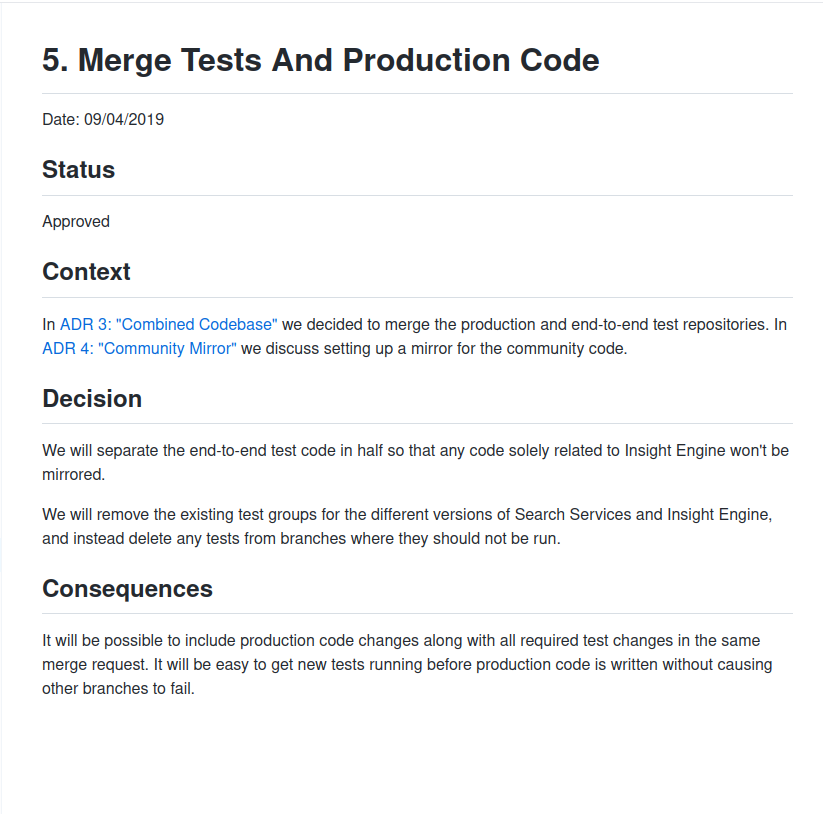
\includegraphics[scale=0.5]{figures/ADR_Example.png}
            \caption{ADR Example used by an open source project using the template format proposed by Michael Nygard}
            \label{fig:ADR_Example_MN}
        \end{figure}

        Numerous other ADR templates have been proposed. Tyree and Akerman's (\textbf{TA}) Template, is one of the first templates proposed that enriches the document with sections such as "Constraints", that reduce the solution space, "Grouping", that states how the new component will tie in to the existing system structure, and an "Argument" section that rationalizes the decision. The markdown ADR (MADR) (\textbf{MD}) template\cite{MarkdownADRs} on the other hand describes the problem as a "User Story", that resembles a ticketing system reference and the decision is motivated by "Decision Drivers". It can also outline the decision alternatives in detail in each separate section. The Alexandrian template pattern (AP) is also a simple document containing solely two sections, an "Introduction", that defines the problem in a summary, the decision made and its results, and a "Specifics" section that gives more context on both the solution, the problem (as a story of the current state of things and the quality of the options considered. The Business Case ADR (BC) template views the document from a perspective of a business analyst that oversees architectural decisions. It focuses on evaluation criteria, candidate solutions, and associated costs. When it comes to sections, it includes a top-level overview of the problem that eventually leads to a recommendation on how to solve it. For each solution candidate, it provides a detailed analysis covering how the candidates were discovered, research methods, criteria fulfillment, cost analysis, SWOT analysis, and internal and external opinions. Lastly, the Planguage (PL) template is more quality assurance oriented. It uses a special informal, but structured, keyword-driven
        planning language that can be used to create rich specification of requirements solely using keywords such as "Tag", "Gist", "Requirement", "Rationale", "Priority", "Stakeholders",  "Author", "Revision", "Date", "Assumptions" in a format that is not separated by sections but instead resembles a database entry that can be indexed efficiently and reducing ambiguity. A detailed comparison of each template along with some of the most common sections mentioned in them can be seen in the table in \ref{table:adr_template_comparison}. Each "+" symbol signifies the presence of the section title of the far left column whereas each "-" signifies its absence in that specific format.  
    
        \newpage
        \begin{longtable}{|m{5cm}|c|c|c|c|c|c|}
            \hline
            % Nygard , Tyree \& Akerman , Alexandrian Pattern, Business Case, MADR , Planguage
            \textbf{Feature} & \textbf{NY} & \textbf{TA} & \textbf{AP} & \textbf{BC} & \textbf{MD} & \textbf{PL} \\
            \hline
            \textbf{Title} & + & + & - & + & + & + \\
            \hline
            \textbf{Status} & + & + & - & + & + & + \\
            \hline
            \textbf{Context/Background} & + & - & + & + & + & + \\
            \hline
            \textbf{Problem/Issue} & + & + & + & + & + & + \\
            \hline
            \textbf{Forces/Decision Drivers} & - & - & + & - & + & - \\
            \hline
            \textbf{Decision} & + & + & + & + & + & + \\
            \hline
            \textbf{Options} & - & - & - & + & + & + \\
            \hline
            \textbf{Solution} & + & + & + & + & + & + \\
            \hline
            \textbf{Consequences
            /Implications} & + & + & + & + & + & + \\
            \hline
            \textbf{Motivation/
            Rationale} & - & + & - & - & + & + \\
            \hline
            \textbf{Assumptions} & - & + & - & - & - & - \\
            \hline
            \textbf{Related Decisions} & - & + & - & - & - & - \\
            \hline
            \textbf{Stakeholders} & - & - & - & - & - & + \\
            \hline
            \textbf{Pros and Cons} & - & - & - & - & + & - \\
            \hline
            \caption{Comparison of ADR Templates}
            \label{table:adr_template_comparison}
        \end{longtable}

        Tool support for creating and managing ADRs is currently limited to few but powerful options. One of the most popular alternatives is "ADR Tools"\footnote{https://github.com/npryce/adr-tools}. It is a command-line utility that is close to the development lifecycle and helps manage ADRs by providing commands to create, maintain, and visualize these records in a project. It has beed rewriten in many programming languages showcasing its popularity. Other tools such as "Loqbooq"\footnote{https://loqbooq.app/} and "adr-manager"\footnote{adr-manager} are web applications focusing on simplicity when managing ADRs, while other libraries such as "Embedded Architectural Decision Records"\footnote{https://github.com/adr/e-adr\#embedded-architectural-decision-records} for Java and "architectural-decision"\footnote{https://github.com/cspray/architectural-decision} for PHP provide the option to embed ADRs inside functional code. The later can also be a viable option for organizations that prefer only writing comments for documenting all aspects related to system code.

    \newpage
    \section{ADRs in practice}
        % Spotify + overview of process if needed
        ADRs have been used in practice and its use endorsed by prominent organizations. One example is Spotify\cite{Spotify_ADRS} that reports benefits such as ease of onboarding of new engineers, since new hires are able to get up to speed with code and system principles faster instead of discovering them as they navigate the challenges of their work. This proves that since ADRs also constitute a piece of AK, they can enhance knowledge sharing across stakeholders and geographically distributed teams (such as those in Spotify) \cite{AK_management} by removing barriers to knowledge management systems. They also report that ADRs enable more efficient ownership handover in organizations that do frequent internal restructuring of departments as they lower the friction of information transferring and allow for a seamless system ownership transition to new teams. Finally they facilitate alignment between different parts of an organization by providing a single source of truth for all architecture related decisions.

        % Redhat
        ADRs are also encouraged by Red Hat\footnote{https://www.redhat.com/architect/architecture-decision-records} especially paired with the Open Decision Framework\footnote{https://opensource.com/open-organization/resources/open-decision-framework} which is a set of best practices developed by Red Hat for making transparent, inclusive decisions in organizations that adhere to open source principles, focusing on collaboration, diverse perspectives, and clear communication. They state that when the architectural decision affects multiple stakeholders, it can be integrated in an ADR feedback loop facilitated by a pull request, focusing on open source principles.  

        % Amazon + overview of process if needed
        Amazon and its cloud service, Amazon Web Services (AWS) also highlight the need of ADRs as key architectural documentation\footnote{https://docs.aws.amazon.com/prescriptive-guidance/latest/architectural-decision-records/} as it "streamlines technical decision-making", by providing a structured process for documenting, justifying, and communicating architectural decisions. They explicitly mention architectural decision repositories as a means of storing such knowledge. Inside AWS, ADRs help align team members with the strategic direction a system may be taking, set general project directions and guidelines, and avoid common decision-making pitfalls by capturing the context, rationale and solutions behind past experiences. Furthermore, they state that ADRs can reduce development time, improve documentation, and enhance the handover process for future teams, ensuring that critical information is preserved and is indexed and accessible. 

        % Github (TODO if needed)


\chapter{Research Methodology}
    \section{Research Approach}
        % General Overview of what was done
        In this study, a mixed-methods approach was adopted to analyze the topics addressed in ADRs from a dataset gathered from GitHub by practitioners. The goal was to uncover patterns and prominent architectural interests within the practitioner community and how those interests relate to the general topics of software architecture. 

        % General overview of how it was done and why it differs from others 
        Specifically, a dataset from a previous mining software repositories (MSR) study on ADRs, that resulted from a systematic process and guidelines, \cite{Github_study_ADRs, MSR_systematic_process} was leveraged to perform analysis on the records' contents using machine learning techniques and empirical observations to interpret and classify the results. While the researchers focused on finding out how widespread the use and adoption of ADRs has become, aiming to uncover the trends and metadata in regards to the ADRs that were mined, this study's objective is to determine the topics of the aforementioned records by getting insights into their contents and architectural fields of interest.

        % Dataset origin and why use it (skipped my modifications of the dataset since they are mentioned in the next chapter)
        The dataset was selected and deemed appropriate for the study for numerous reasons. Firstly, because of the recency of the data, dating back to 2020, four years before the present study was conducted. Secondly, because of the platform used to derive the dataset, as GitHub is the largest platform for open source software repositories by a significant margin\footnote{https://osssoftware.org/blog/open-source-software-repository-management/}. Lastly, because of the dataset quality and quantity, as it derived from an exhaustive automated search of all publicly available repositories  (estimated 128,411,417 as of February 26 2020\footnote{https://github.com/bugout-dev/mirror/blob/master/notebooks/rise-of-github.ipynb}) and the selection process was strict, involving manual and automated screening of results, applying concrete inclusion and exclusion criteria to identify repositories actually using ADRs for documenting ADDs, while excluding those with low quality documents.

        % Methods of analysis and why i used them
        For the identification of prevalent topics within the records' contents, a number of techniques were used, focusing on machine learning approaches applied using automated methods in Python. In detail, topic modeling, a text mining technique, was utilized for its effectiveness to extract abstract topics and word clusters from a collection of documents. This method was employed as it has also demonstrated efficacy in other software engineering empirical studies, analyzing text mostly related to developer communication and bug reports \cite{Topic_modeling_in_software_engineering_research}. Approaches using Latent Dirichlet Allocation (LDA) were also employed as they constitute common practice in the topic modelling space, with mixed results. Combining all the findings, a specific stack of algorithms and techniques was chosen, described in detail in the following chapters and facilitated by the use of the BERTopic Python library \cite{bertTopic}.

        % Result interpretation
        To interpret the analysis results, multiple approaches were utilized as there is no definitive method to objectively label topic clusters, which also depends on the reader's perspective \cite{datasciencecentralTopicModeling}. In the absence of ground truth, keywords from the record clusters were analyzed and interpreted using large language models (LLMs) as representation models. The labels were then cross-checked with the most representative documents of each cluster, specifically those that are semantically closest to the center of the cluster based on their distance in the vector space. Additionally, in certain cases, manual topic naming was performed based on frequent words within a topic, a common practice in topic modeling to reduce ambiguity \cite{Topic_modeling_in_software_engineering_research}.
        
    \section{Research Objectives and Questions}
        As mentioned, The main objective of this study is to uncover prominent software architecture topics by examining a collection of ADRs. To achieve those research objectives,the following research questions were defined (RQs):

        \begin{itemize}
            \item \textbf{RQ1}: What are the most frequently discussed software architecture topics in ADRs?
            \item \textbf{RQ2}: Which topics from the general software architecture space are present in the ADRs?
            \item \textbf{RQ3}: Which ADR topics cannot be classified, and what are the reasons behind this? 
        \end{itemize}. 

        The aim of RQ1 is to outline the most prevalent topics that concern open source maintainers and owners of the repositories whose ADRs are being analyzed, effectively examining the most common design decisions projects face.
        
        RQ2 aims to compare the identified topics with various aspects of software architecture to determine if they are aligned. This comparison could also provide insights into less prevalent software architecture topics as well as the breadth of the ADRs in the dataset and suggest future directions for enriching it.
        
        Finally RQ3, aims to discover the intricacies that outlier ADRs might have. This, on the one hand may help discover new architectural concerns or interesting architecture sub-domains that have not been yet thoroughly researched. On the other hand, it could also just discover ADRs that talk about topics too niche to be considered, validating potential suspicions about their irrelevance.

\chapter{ADR Dataset and Extraction}

    \section{Data collection Process}
        The dataset used for the study was obtained from a previous MSR study\cite{Github_study_ADRs}. The researchers preformed an exhaustive search on GitHub in 2020 which included going through all registered platform users to find public repositories that contained files that matched various template formats of ADRs. After this process was completed, the repositories were also verified manually according to rigorous inclusion and exclusion criteria. The resulting dataset contained metadata for 6362 ADRs from 921 software repositories. However, since the researchers focused mainly on measuring trends and use of ADRs, only the metadata were stored and made publicly available in a separate GitHub repository\footnote{https://github.com/software-competence-center-hagenberg/ADR-Study-Dataset}. The dataset files, one for each repository, were stored in a JSON format and contained information about the repository such as its hyperlink, the number and path of ADR directories, and detailed metadata for each ADR as seen in figure 5.1\ref{fig:JSON_data}. This metadata included the directory path, file path, type of ADR template used, status, timestamps of the first and last commits, the number of commits, and details about the authors. Because of the need to focus on the contents of each ADR, each repository needed to be cloned (downloaded) and the ADRs to be extracted from the specified folder as mentioned in the metadata. This also accounted for newly created ADRs after the date the data was scrapped since the projects may have continued their use even after the study was published. It is important to note that some GitHub repositories (~20) were deleted, which prevented their inclusion in the dataset. The whole was done in an automated way via a Python script. The final contents of the respective folders were saved and examined.

        \begin{figure}[]
            \centering
            \includegraphics[scale=0.4]{figures/JSON_data_example.png}
            \caption{Example of a JSON metadata file derived from the base dataset.}
            \label{fig:JSON_data}
        \end{figure}
        
    \section{Data Cleaning and Enrichment}
        After the contents of the ADR folders were obtained, at first, the files needed to undergo a cleaning process. I decided to include only markdown files since they comprised the vast majority of the actual files downloaded at a percentage of more than 98 percent and was the dominant file type for the ADRs as proposed in the Markdown Architectural Decision Records \cite{MarkdownADRs} article. This also eliminated exogenous files such as any source code that was stored in the folders in question. Next, irrelevant files and files related to ADRs that did not provide any actual information of use needed to be deleted such as licences, ADR templates, contributing guides and "README" files. ADR drafts and examples were also excluded since they did not relate to any specific topic. This procedure was also executed automatically via Python scripts and it resulted in 5368 ADRs markdown files.

        The final cleaning process was performed on the ADR text itself to reduce language-dependent factors in order for the topic modelling analysis to produce more coherent results. Text is generally written in natural language for human understanding, but in text mining, this data is not always straightforward for computers to process as it frequently contains words and other elements that provide no information gain to algorithms and models. Therefore, it is common practice in topic modelling, for text to undergo preprocessing where specific tokens from documents are usually removed. \cite{topic-modelling-text-cleaning, text-mining-lda}. In this case, all non-alphabetic characters were removed and all text was converted to lower case. In addition, stop words, stemmed from the ntlk natural language toolkit Python library were also removed as they were deemed insignificant. These included pronouns in many forms from a commonly used list of 127 entries\footnote{https://gist.github.com/sebleier/554280}. Furthermore, all words with less than 3 characters were also filtered out and all remaining words were lemmatized or reduced to their base or root form, by removing inflections and derivational suffixes, ensuring that related forms of a word are treated as a single item. Finally, a list of unwanted terms was manually assembled after careful examination of a subset of documents. This list included words from common ADR template titles such as "context", "decision", "status", "consequences", "motivation", "options", "option", "alternatives" and others, that were present in almost all documents and did not provide any context on their topics, but instead were used to honor the ADR format. Other common but unwanted words included the name of the proposer of a popular ADR template "Michael Nygard" \footnote{https://cognitect.com/blog/2011/11/15/documenting-architecture-decisions} and were also filtered out. Code-specific stopwords such as "class," "interface" and "abstract" were not removed as to provide information about the implementation of the decision. The final form of each document was reduced to a series of words that captured the semantic properties and general meaning of the architectural decision. An example cleaned ADR can be seen in figure \ref{fig:Cleaned_ADR} and an overview of the cleaning process in figure \ref{fig:Data_cleaning_steps}
        
        \begin{figure}[]
            \centering
            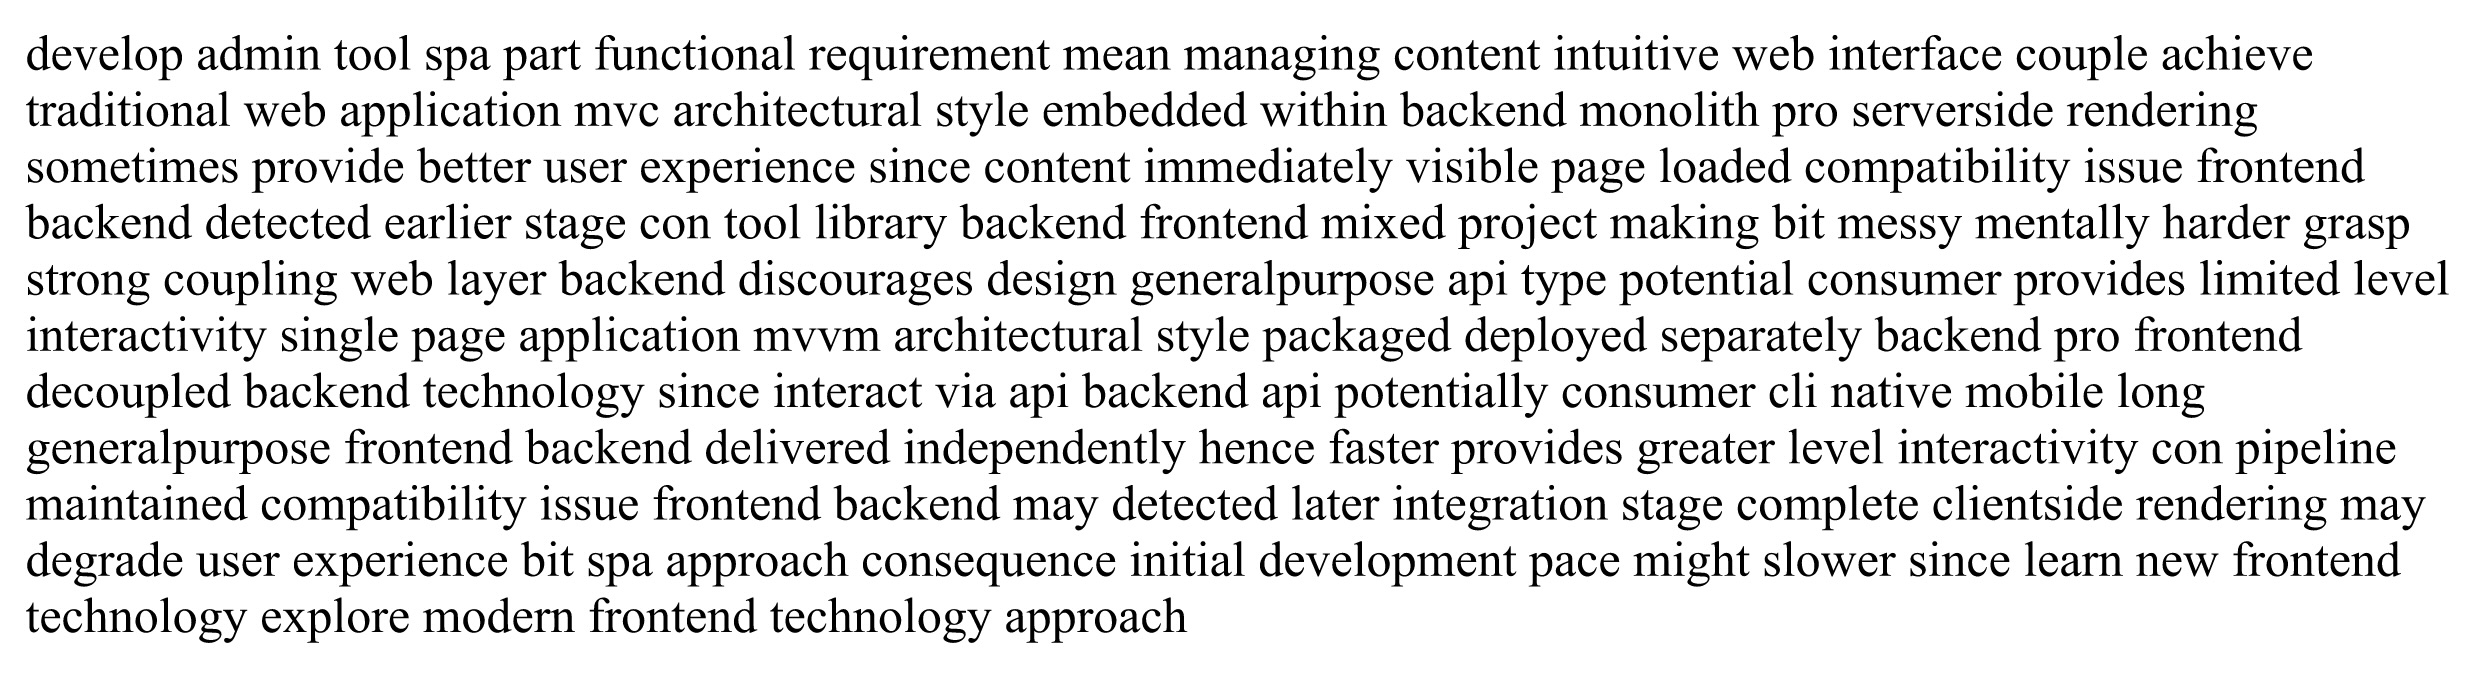
\includegraphics[scale=0.6]{figures/adr_cleaned_example.jpeg}
            \caption{Example of an ADR about creating a web interface after undergoing preprocessing.}
            \label{fig:Cleaned_ADR}
        \end{figure}

        \begin{figure}[ht]
            \centering
            % \fontsize{7}{8}\selectfont
            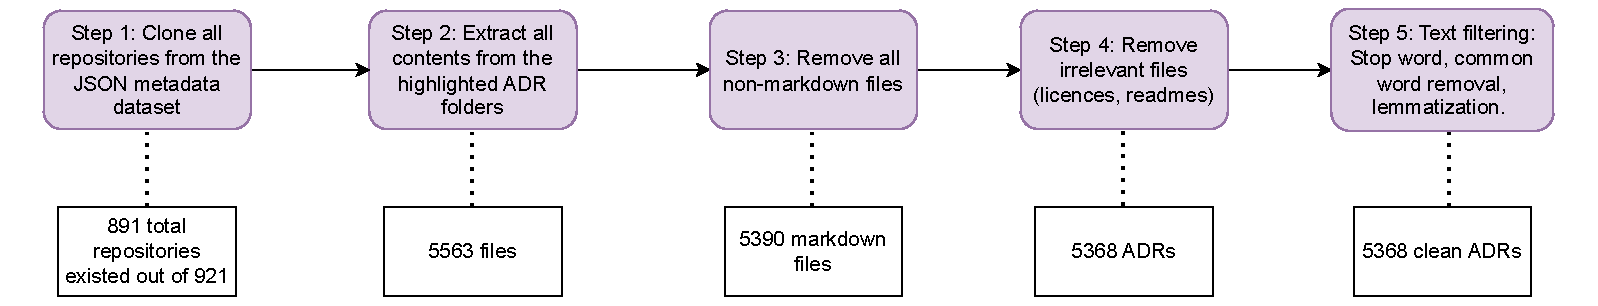
\includegraphics[width=\textwidth]{figures/data_cleaning_steps_final2.pdf}
            \caption{Data cleaning process.}
            \label{fig:Data_cleaning_steps}
        \end{figure}
        
    \section{Dataset Validity and Quality}
    While this dataset provides a valuable snapshot of ADR usage in open-source projects, several validity and quality concerns need to be addressed. Firstly, despite it being derived from a broad search on all GitHub repositories, the final sample size remains small. There exist a plethora of reasons for why this may be observed. ADRs are not yet widely adopted, which is understandable since they were introduced recently, with the earliest ADR commit in the dataset dating back to May 2013. Furthermore, it is possible that many ADRs remain private, either in private code repositories or internal company documentation, not found on any code hosting platforms. The later can be confirmed by the statements of companies like Spotify and Amazon, as mentioned in chapter 3, that choose to keep code proprietary and records private.
    In addition, in regards to ADR content and selection, potential over-filtering might have removed relevant information, and the manual assembly of unwanted terms introduces an element of subjectivity. In contrast, it is possible that records and phrases that provide no additional meaning were not filtered and a more thorough approach of examining the records before cleaning them is needed. To promote dataset quality, future research could include expanding the dataset size with private records, or public ADRs that are not stored on GitHub and refining the cleaning process to mitigate these limitations.

\chapter{ADR Dataset Analysis}
    For the analysis of the ADRs, and to answer the research questions, several topic modelling techniques and algorithms were used as mentioned in chapter 4. This section presents the two approaches that led to the final results.
        
    \section{Analysis Using TF-IDF and LDA}
        A fist approach employed Term Frequency-Inverse Document Frequency (TF-IDF) for vectorization of words and Latent Dirichlet Allocation (LDA) to perform the topic modelling. TF-IDF is a statistical measure used to evaluate the importance of a word in a document relative to a collection of documents. By applying TF-IDF, each document is converted into a numerical vector, where each element of the vector represents the TF-IDF score of a term, which in extension is essentially the product of TF, the frequency of a a term appearing in a document and IDF, a metric of importance of the term across all documents. After documents have been vectorized, we can apply LDA which is is a generative probabilistic model that assumes documents are mixtures of topics and topics are mixtures of words\cite{LDA_paper}. LDA assumes each document is generated from a fixed number of topics, and each topic is a distribution over a certain fixed vocabulary. The result of this method is a distribution of topics for each ADR, indicating the prevalence of each topic within itself. TF-IDF is used since LDA expects the input in the form of integers and TF-IDF accomplishes just that, along with encoding information about words in the documents. hyper parameter tuning using grid search was performed to obtain the best parameters, namely max features of TF-IDF, the optimal number of LDA components, and lda learning decay. This resulted in four broad topics discovered. The topics were projected in a 2 dimentional space and visualized in \ref{fig:LDA_results}. All algorithms were executed using Python and visualized using the pyLDAvis library. When interpreting topics, the top ten words by frequency in each cluster were used.

        \begin{enumerate}
            \item 34.98\% of the documents were represented with the following most common words: data, api, user event, service, type, message, request, object, client. This topic is broad and could potentially revolve around decisions about how APIs manage, process, and integrate data. This is topic (a) in figure \ref{fig:LDA_results}.
            
            \item 32.62\% of the documents were represented with the following most common words: test, component, code, project, library, file, framework, version, package, change. This topic seems to revolves around decisions on the processes, tools, and practices involved in software testing and development. This is topic (b) in figure \ref{fig:LDA_results}.
    
            \item 25.51\% of the documents were represented with the following most common words: aws, service, environment, docker, cluster, container, image, kubernetes, cloud, deployment. Based on these results this topic is more clear and revolves around decisions about cloud infrastructure containers and container orchestration. This is topic (c) in figure \ref{fig:LDA_results}.
    
            \item 6.89\% of the documents were represented with the following most common words: record database search architecture adrs architectural markdown elasticsearch index document adr article. This topic is more intertwined and seems to contain ADRs avout the use of ADRs and database decisions. This is topic (d) in figure \ref{fig:LDA_results}.
        \end{enumerate}

        \begin{figure}[hbt!]
            \begin{subfigure}{.475\linewidth}
              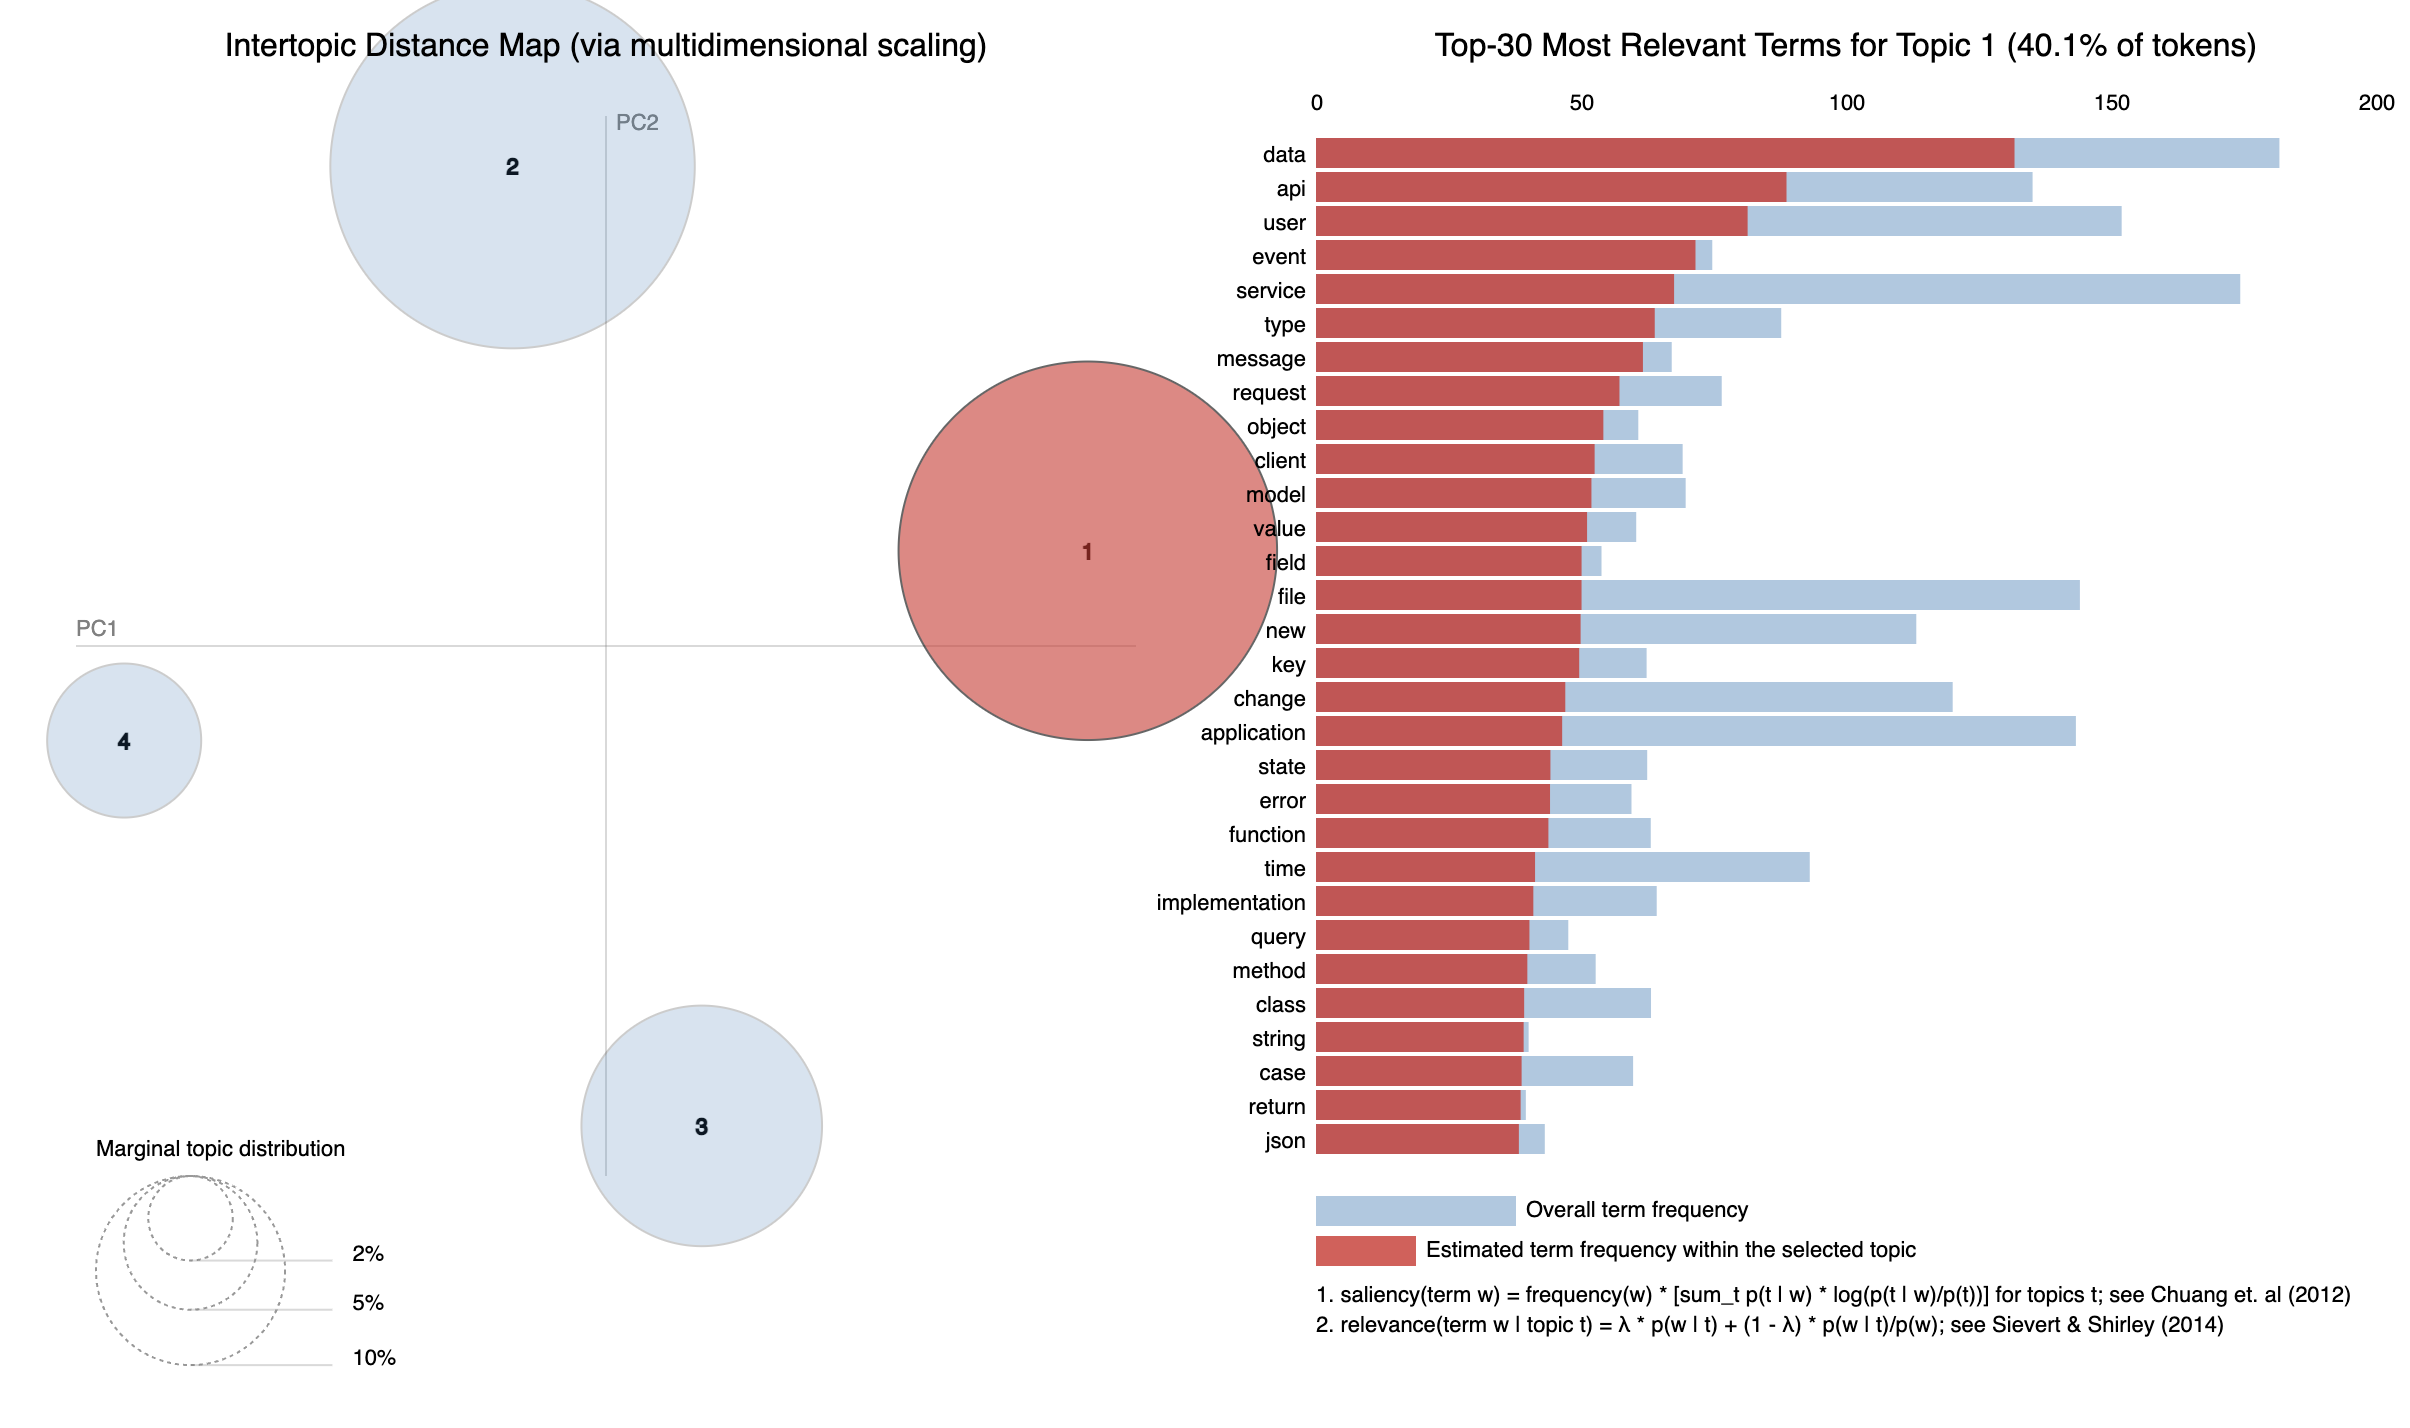
\includegraphics[width=\linewidth]{figures/LDA-results/topic1.png}
              \caption{LDA topic 1}
              \label{MLEDdet}
            \end{subfigure}\hfill % <-- ``\hfill``
            \begin{subfigure}{.475\linewidth}
              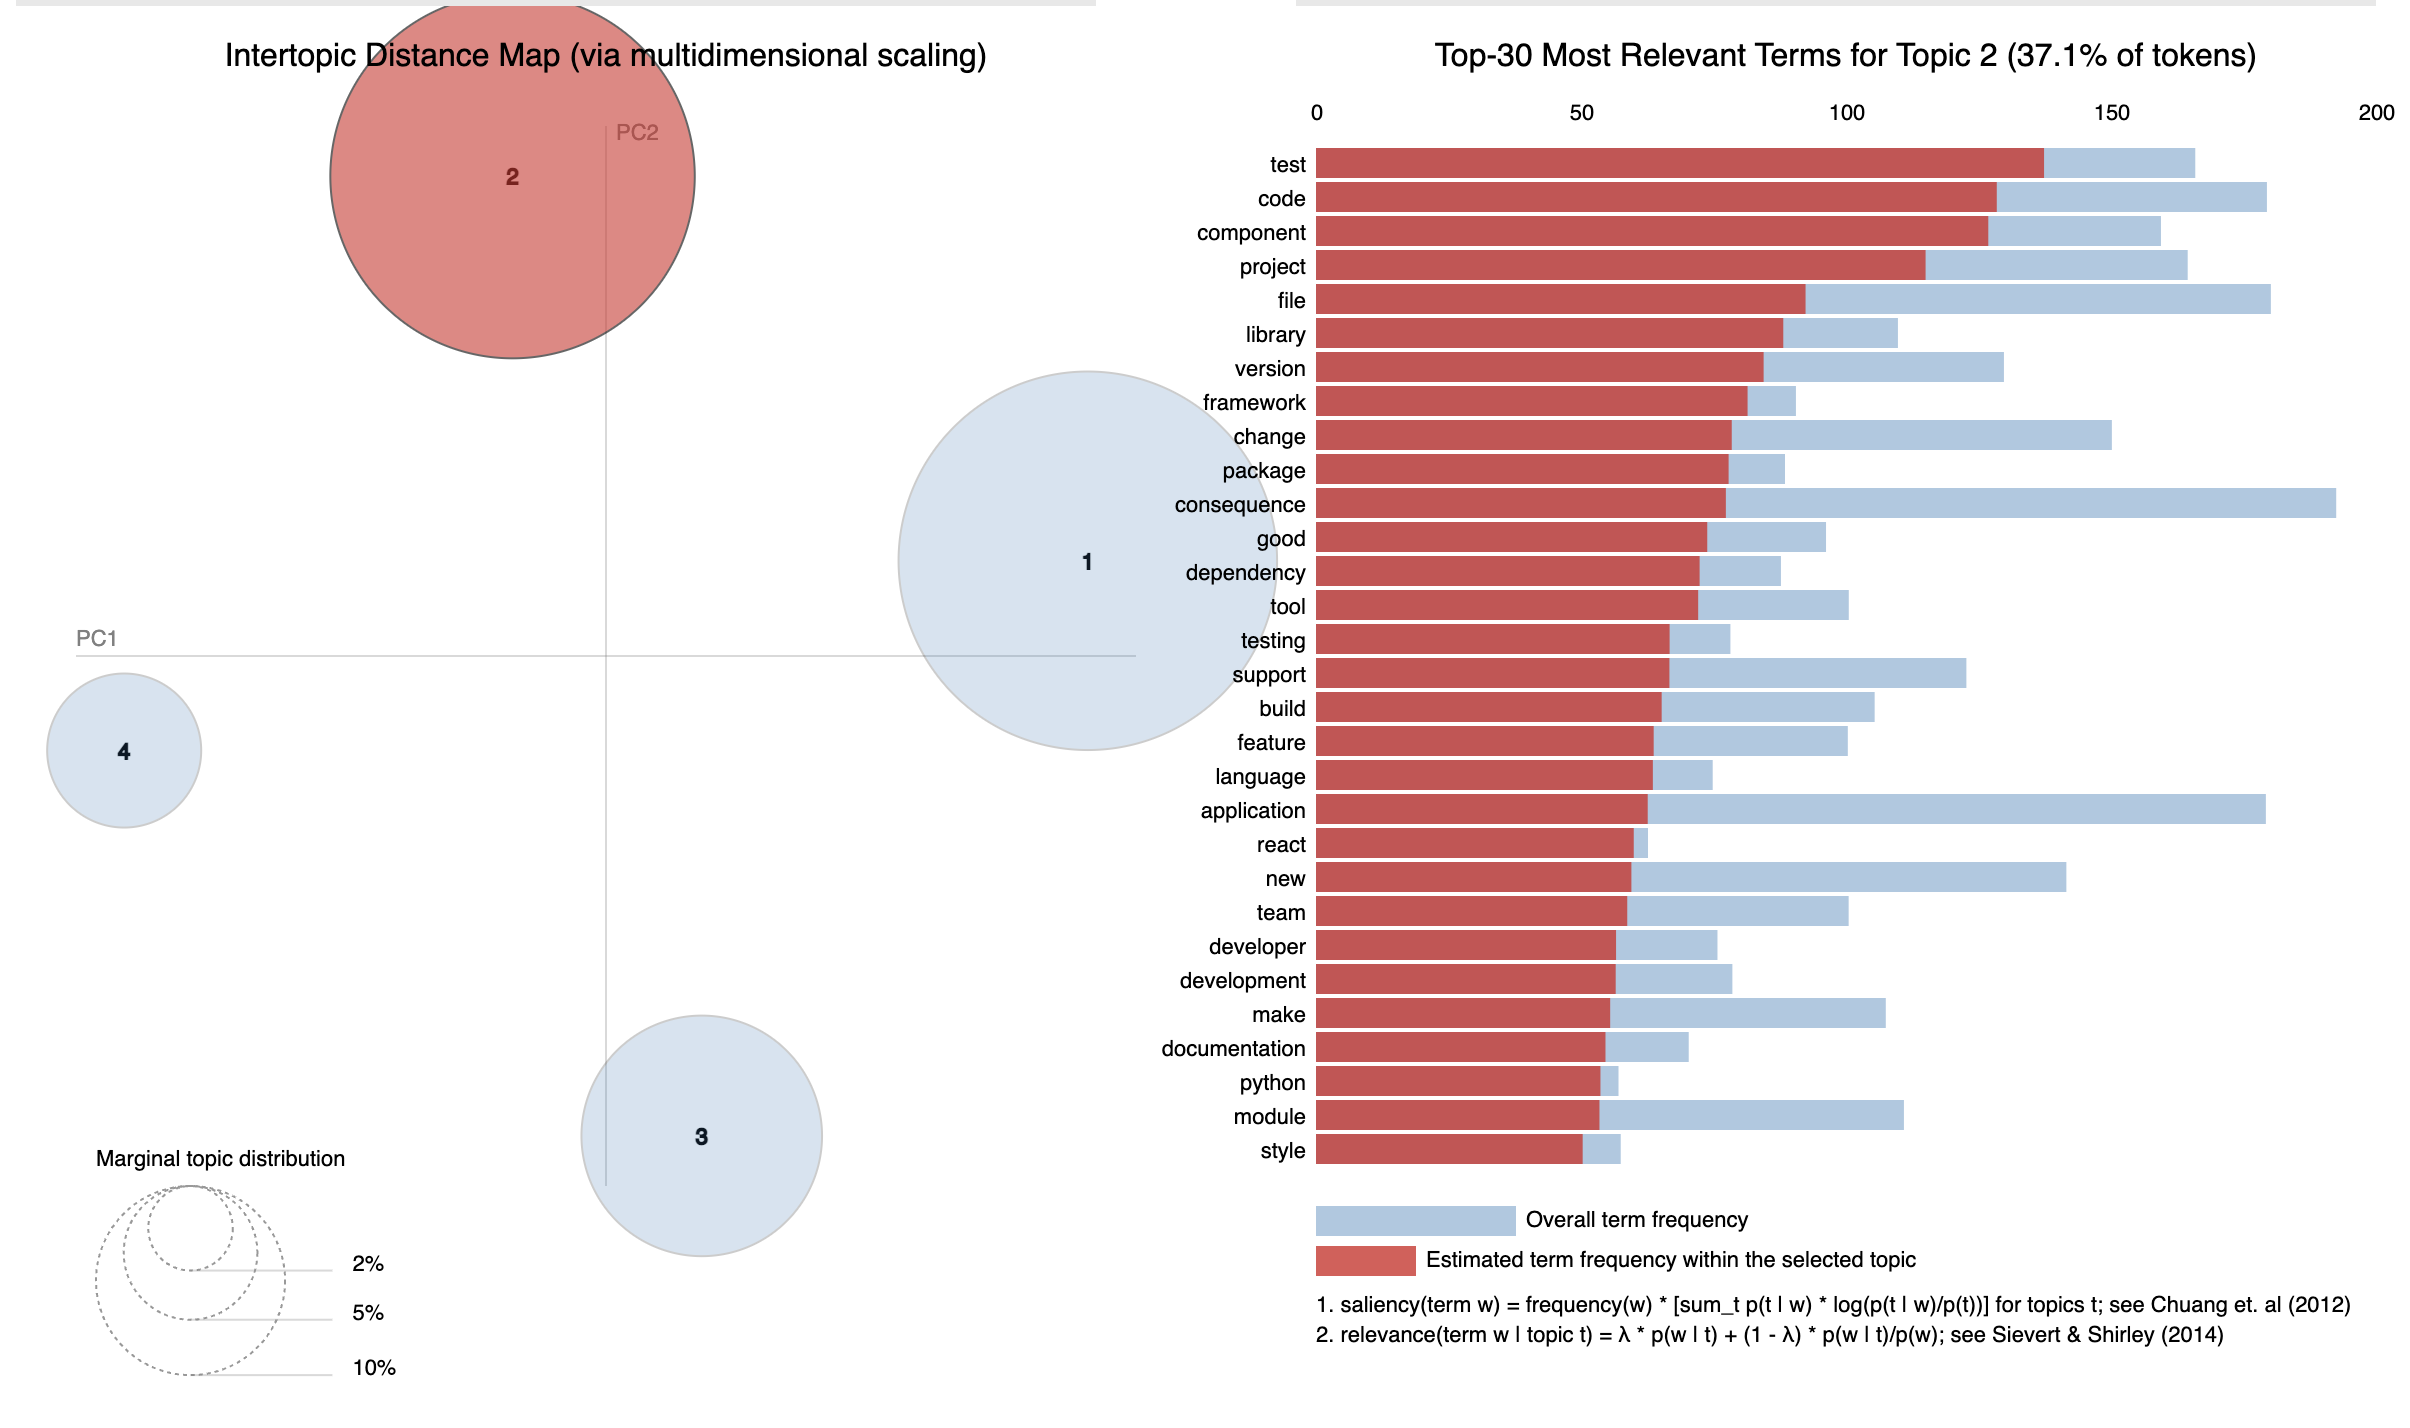
\includegraphics[width=\linewidth]{figures/LDA-results/topic2.png}
              \caption{LDA topic 2}
              \label{energydetPSK}
            \end{subfigure}
            \medskip % create some *vertical* separation between the graphs
            \begin{subfigure}{.475\linewidth}
              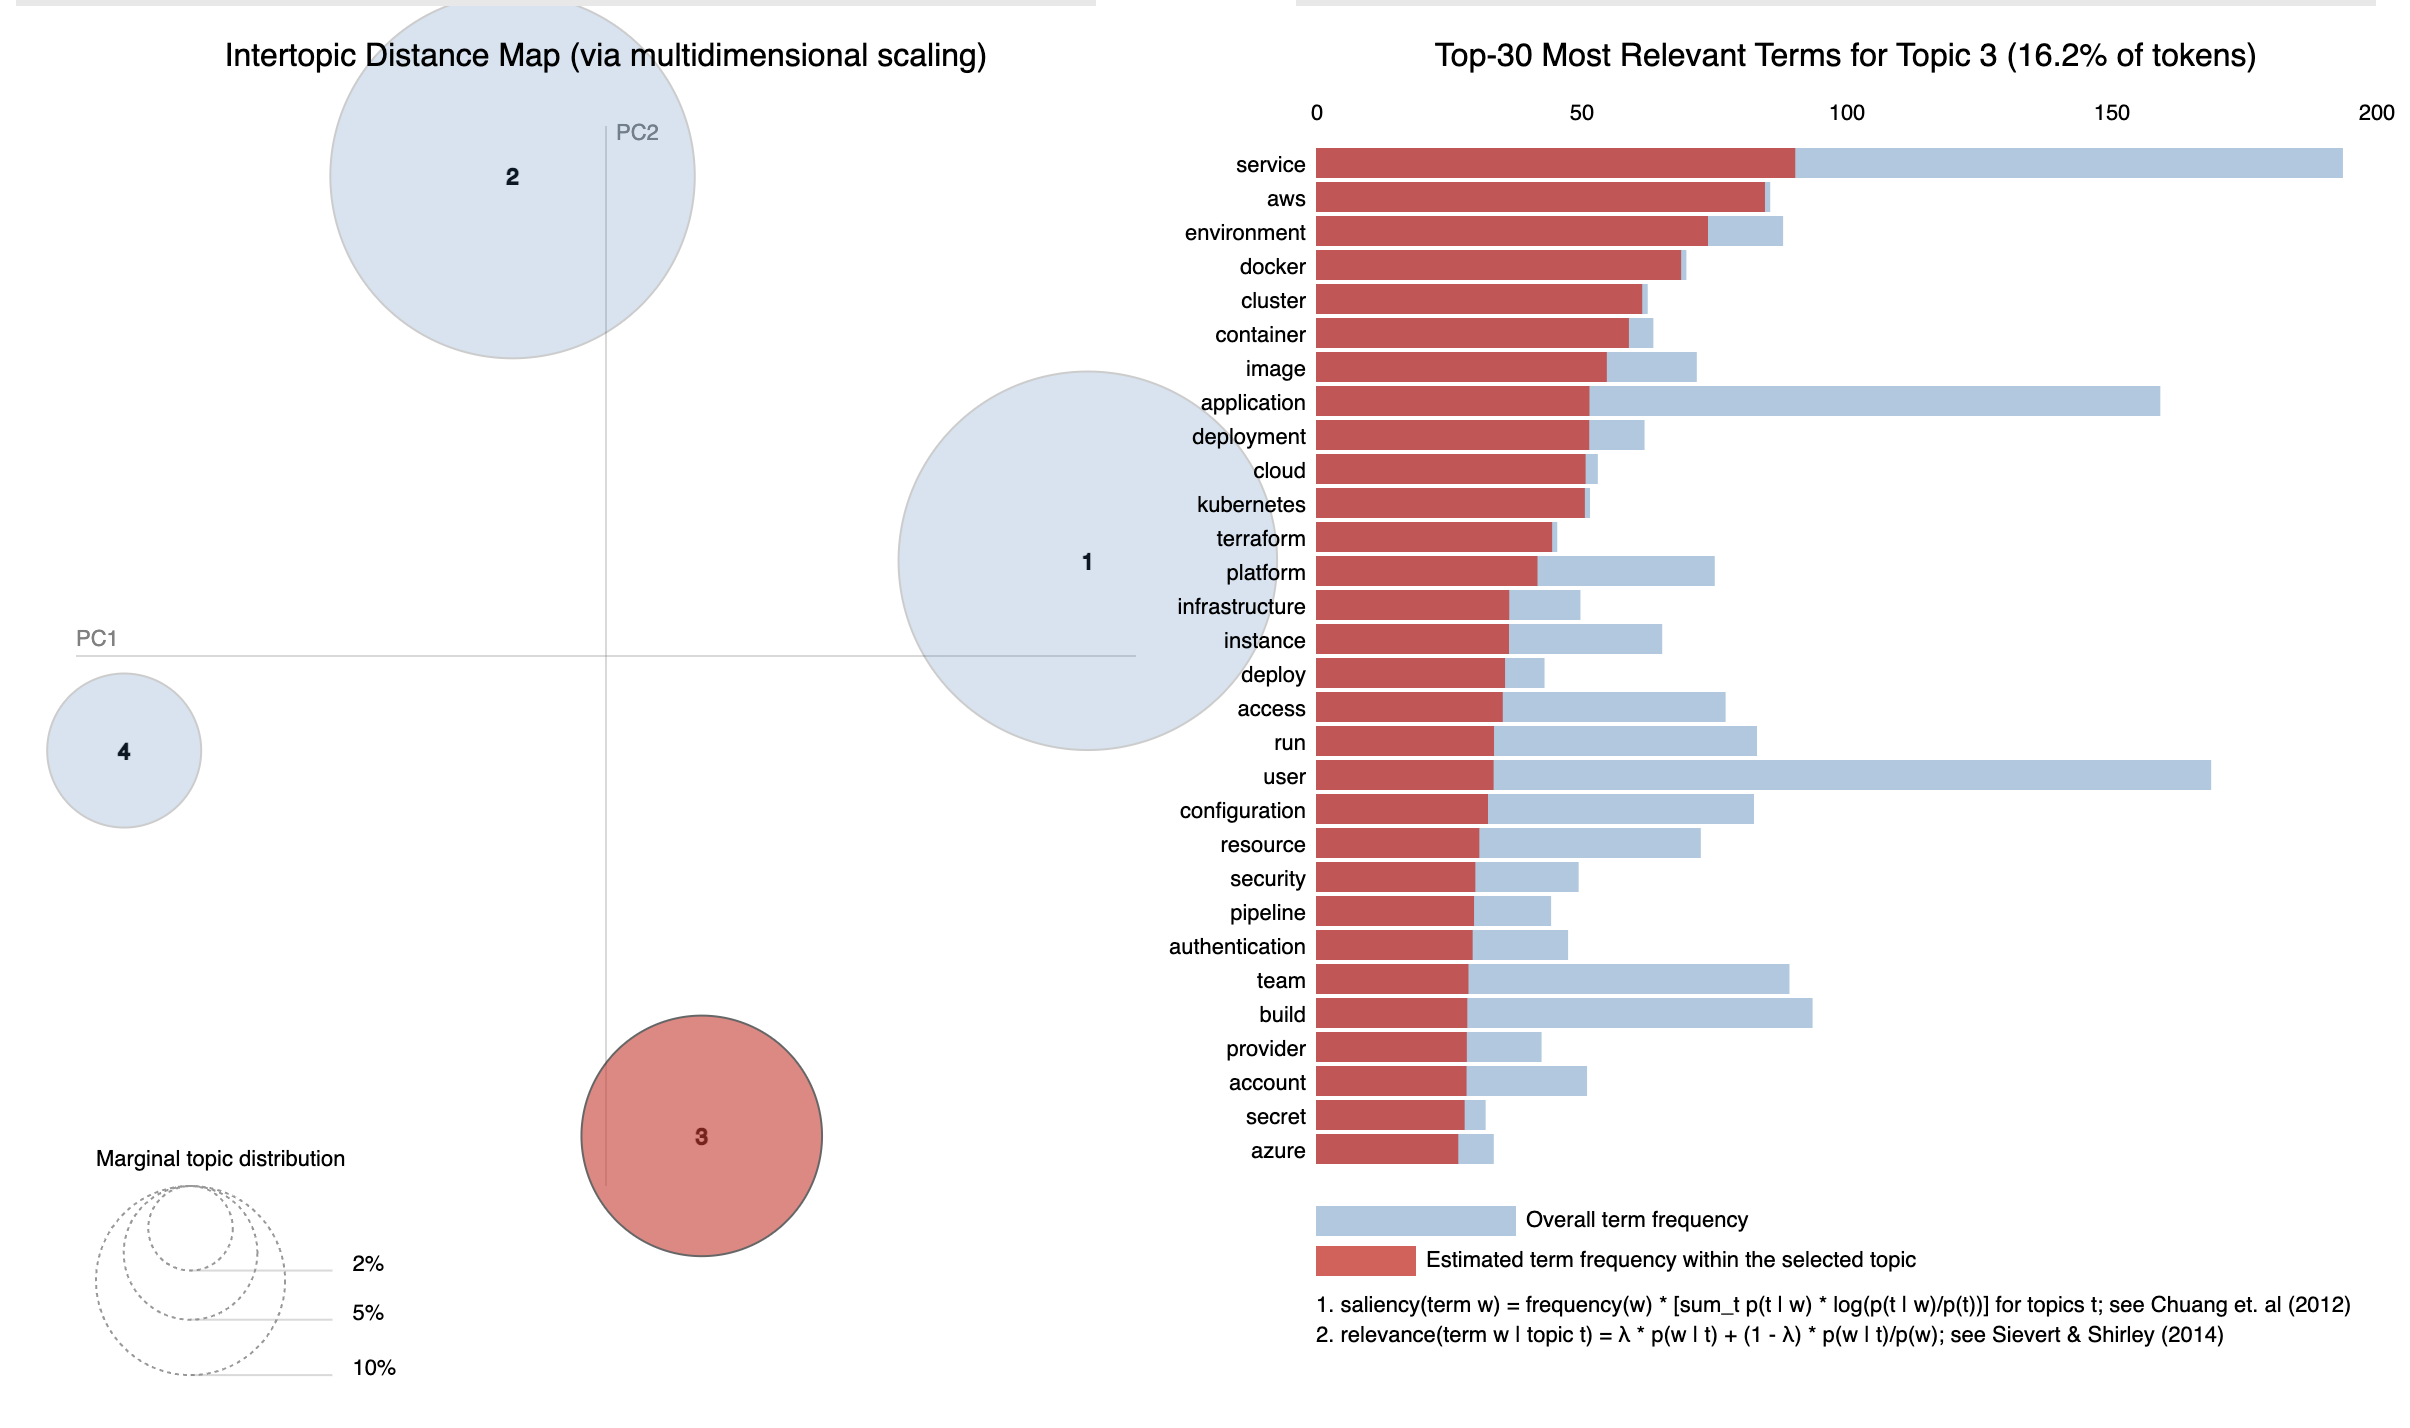
\includegraphics[width=\linewidth]{figures/LDA-results/topic3.png}
              \caption{LDA topic 3}
              \label{velcomp}
            \end{subfigure}\hfill % <-- ``\hfill``
            \begin{subfigure}{.475\linewidth}
              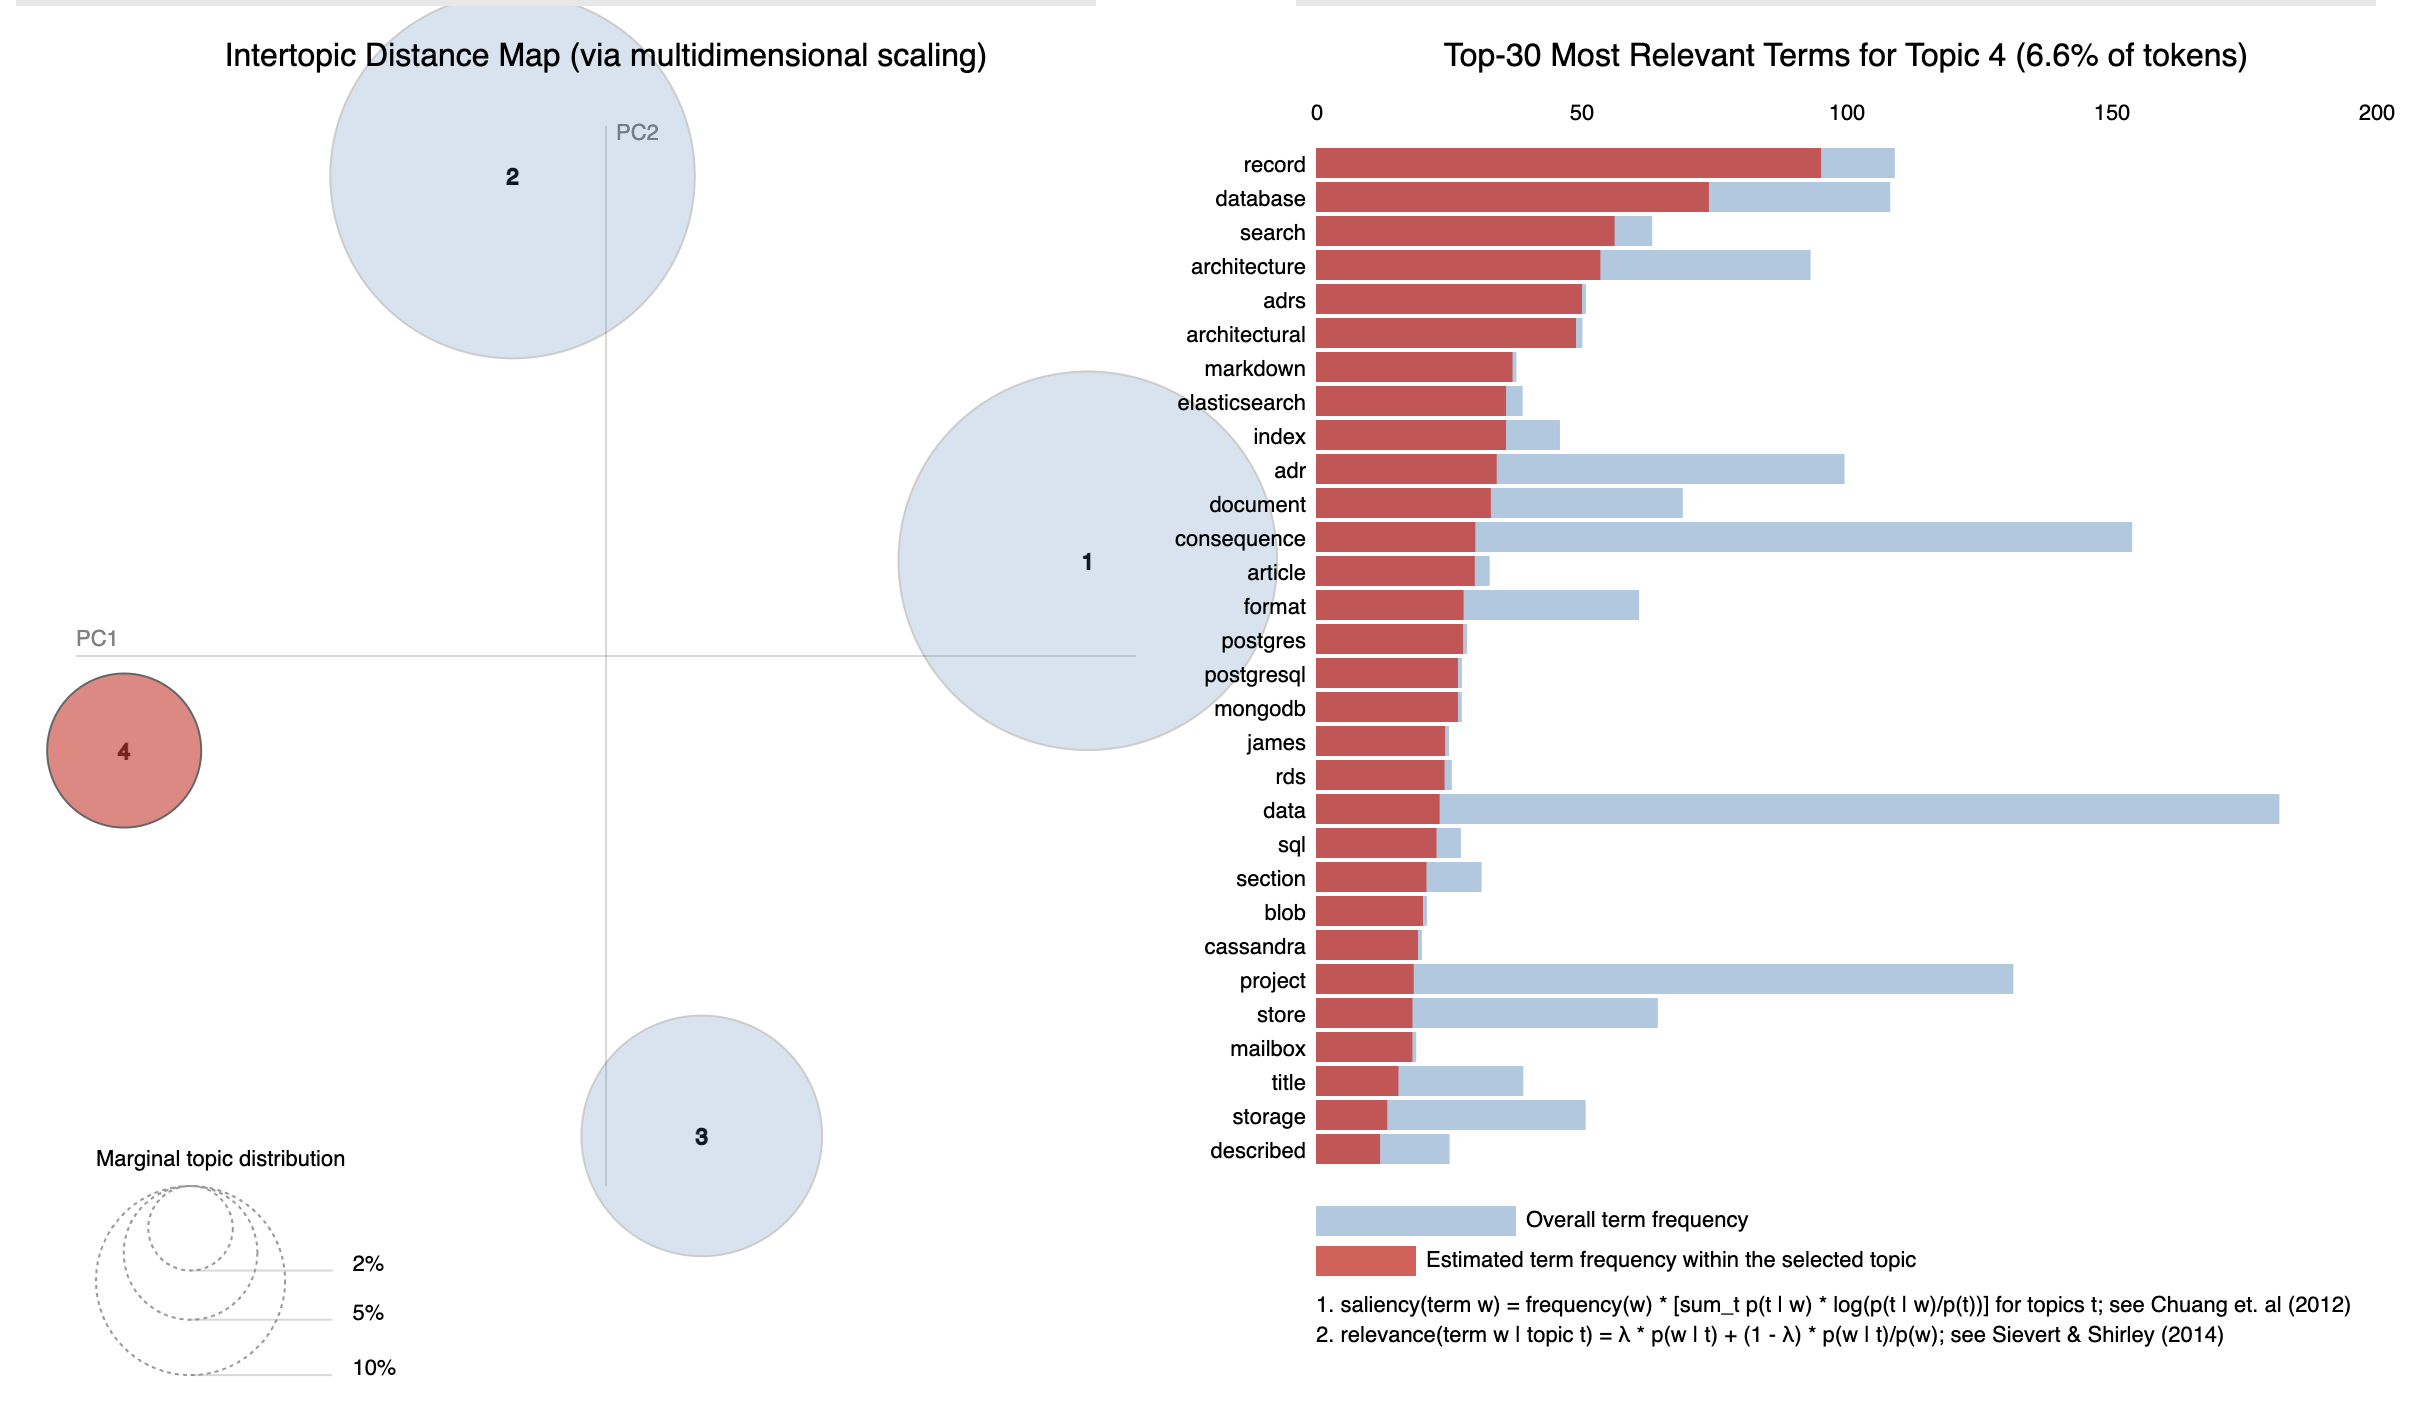
\includegraphics[width=\linewidth]{figures/LDA-results/topic4.png}
              \caption{LDA topic 4}
              \label{estcomp}
            \end{subfigure}
            \caption{LDA topic results with representative words for each topic}
            \label{fig:LDA_results}
        \end{figure}

        LDA served as the base for some further exploration and optimization of employed techniques. While the initial topics generated were not entirely clear, they highlighted the necessity for finer categorization into more specific topics that LDA alone could not effectively capture, even after tuning with many parameter combinations. This was evident as attempting to increase the number of topics resulted in significant noise and incoherence. To address this, other models were introduced and applied, presented in the following subsection.

    \section{Analysis Using BERTopic}
        The second approach utlilized the Python library BERTopic \cite{bertTopic} to analyze the contents of the ADRs. BERTopic uses transformer-based language models and a class-based TF-IDF variation to generate coherent topic representations. The whole procedure and the algorithms used for the final analysis can be broken down to the steps below:

        \begin{enumerate}
            \item Document embeddings are generated using pre-trained models to capture semantic similarities, ensuring that documents with similar topics are close in vector space. In order to produce rich embeddings, the ``all-mpnet-base-v2`` transformer model \footnote{https://huggingface.co/sentence-transformers/all-mpnet-base-v2} from Hugging-Face was used for its support of longer documents up to sequences of 512 tokens and due to the fact that it was trained on datasets related to software engineering such as CodeSearchNet\footnote{https://huggingface.co/datasets/code-search-net/code\_search\_net}, that contains over 2 million (comment, code) pairs and StackExchange questions.
            
            \item These embeddings are then reduced in dimensionality to make the clustering process more efficient. For this, the UMAP method was used as it ``keeps some of a dataset's local and global structure``\footnote{https://maartengr.github.io/BERTopic/algorithm/algorithm.html\#2-dimensionality-reduction} which is important to keep as it contains the information necessary to create clusters of semantically similar documents. This technique introduces randomness into the procedure so a set seed was used to make results reproducible.

            \item Clustering is then performed with the reduced embeddings to separate the documents. For this, HDBSCAN was used. This technique was chosen as it can handle varying densities and can also identify outliers, that do not get assigned to a particular topic. Information of this kind is useful for RQ3. The minimum cluster size hyperparameter, which is the main determinant for the number of  topics the model identifies, was set to 40 or about one\% of total ADRs, as smaller numbers produced very distributed niche topics, that related to specific technologies or tools without providing much information about the context or architecture. A larger minimum cluster size on the other hand, produced incoherent clusters without clear separation.

            \item A bag-of-words representation is then created using all documents in the clusters by counting how often each word appears in each collection. This is important since popular words at the cluster level are needed for the analysis. 

            \item Finally, from the generated bag-of-words representation, TF-IDF is applied again, at a cluster level highlighting important words within a cluster and producing a label. Since we now have a set of representative words for each cluster along with the associated documents a fine-tuning technique was used using OpenAI's model GPT-3.5. Specifically, using a custom prompt, the main set of words for each cluster along with the four documents closest to the center of the cluster were passed as input to the LLM, prompting it to generate characteristic labels for this cluster using natural language. The prompt also contained context of the analysis, stating that the document collection consisted of ADRs, which are part of software engineering.
            
        \end{enumerate}
        
        
    \section{Analysis Results}
        The first form of the analysis' results are presented in figure \ref{fig:bertopic_datamap_original}.

        \begin{figure}[h]
            \centering
            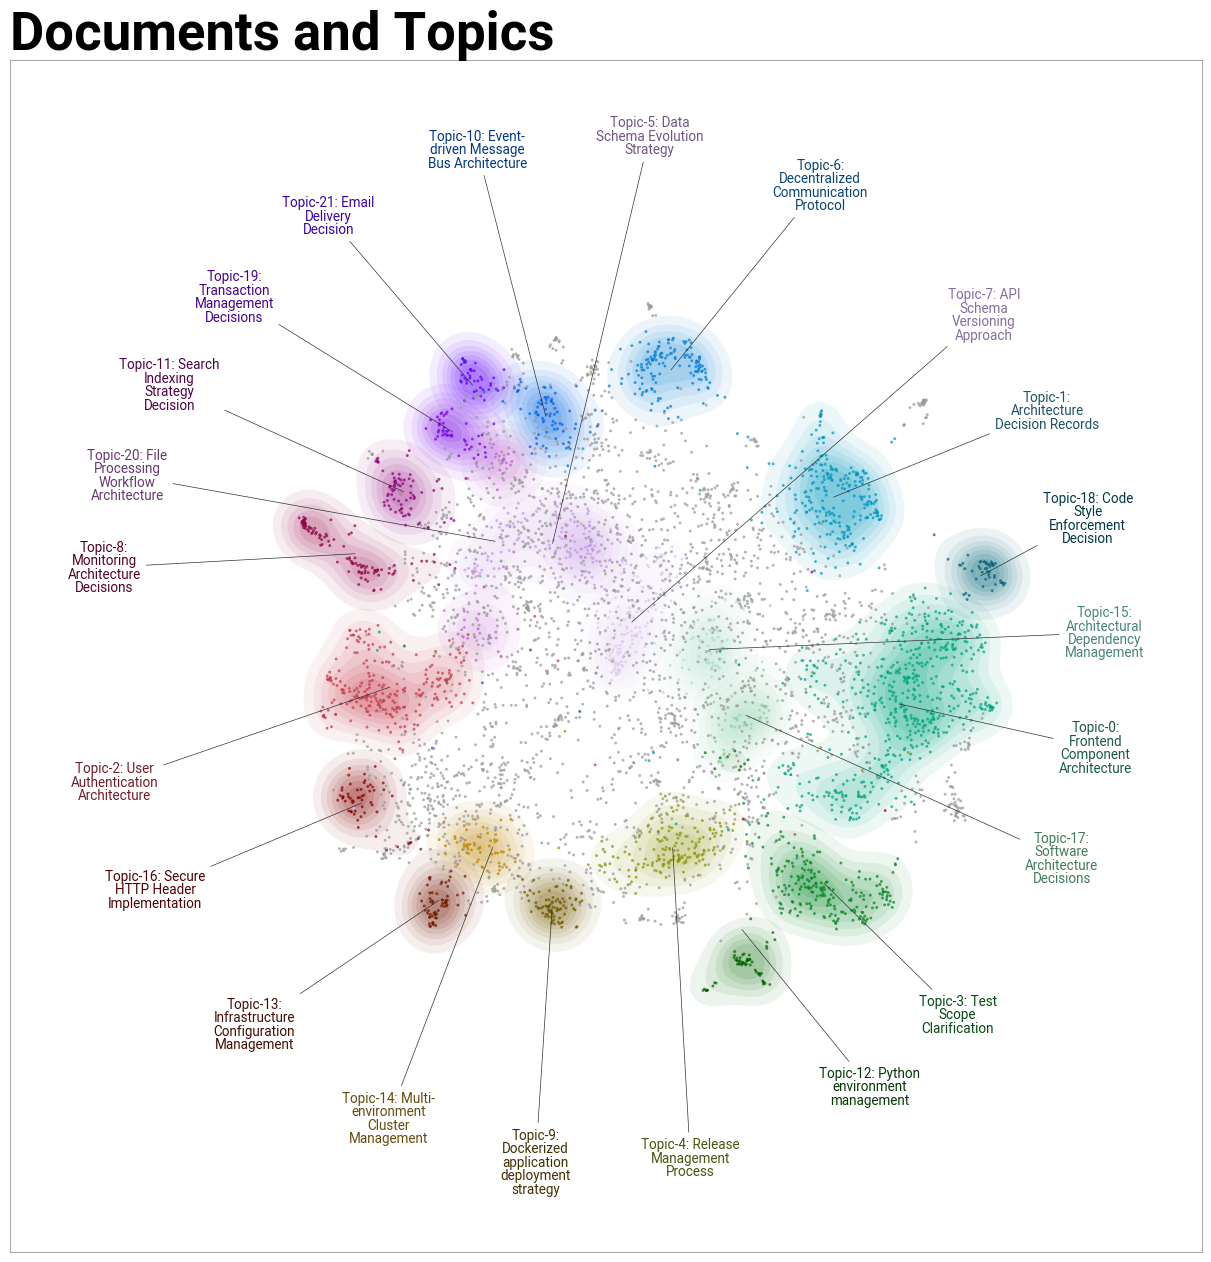
\includegraphics[scale=0.5]{figures/BerTopic_Original/datamap_original.png}
            \caption{Datamap of documents from BerTopic analysis}
            \label{fig:bertopic_datamap_original}
        \end{figure}
        
        In the graph, documents' embeddings are projected in a two dimensional space with each data point representing one ADR. Clusters of documents are highlighted in different colors and their label is the result of the LLM representation model. 22 topics were identified based on the specified parameters. Around 15 of them are formed in tight clusters with clear semantic separation from the others. Those are mostly located around the edges of the graph. However, in the center of the graph, results are ambiguous and clusters are sparse. It is also important to note that 2575 ADRs, highlighted in grey in the center of the datamap, were not able to be assigned to a specific topic. Taking a closer look at the documents themselves by zooming in figure \ref{fig:docs_original}, the center also appears sparse with many documents that have not been classified. 
        
        \begin{figure}[h]
            \centering
            \hspace*{-2.2cm} 
            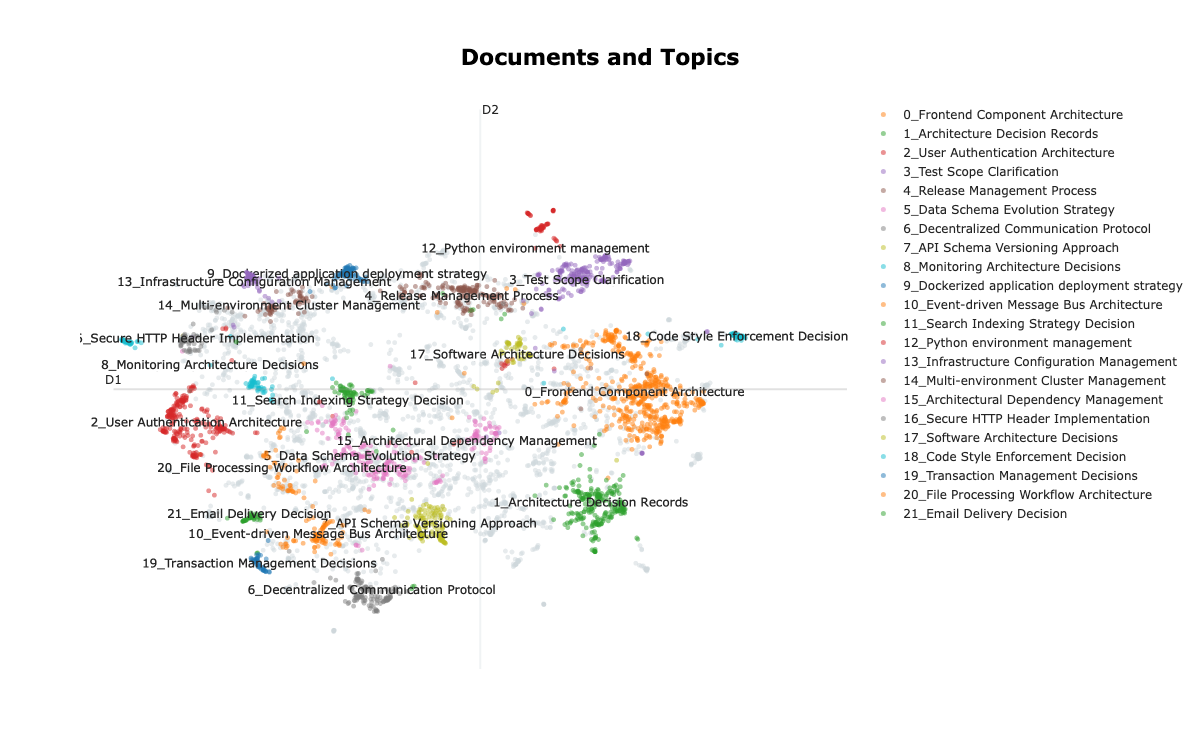
\includegraphics[scale=0.65]{figures/BerTopic_Original/docs_original.jpeg}
            \caption{Document embedding representation from BerTopic analysis}
            \label{fig:docs_original}
        \end{figure}
        
        However, the model seems to have captured semantic similarities in ADRs that serve a clear purpose, especially in certain areas like infrastructure management as presented in in figure \ref{fig:infra_docs}.

        \begin{figure}[h]
            \centering
            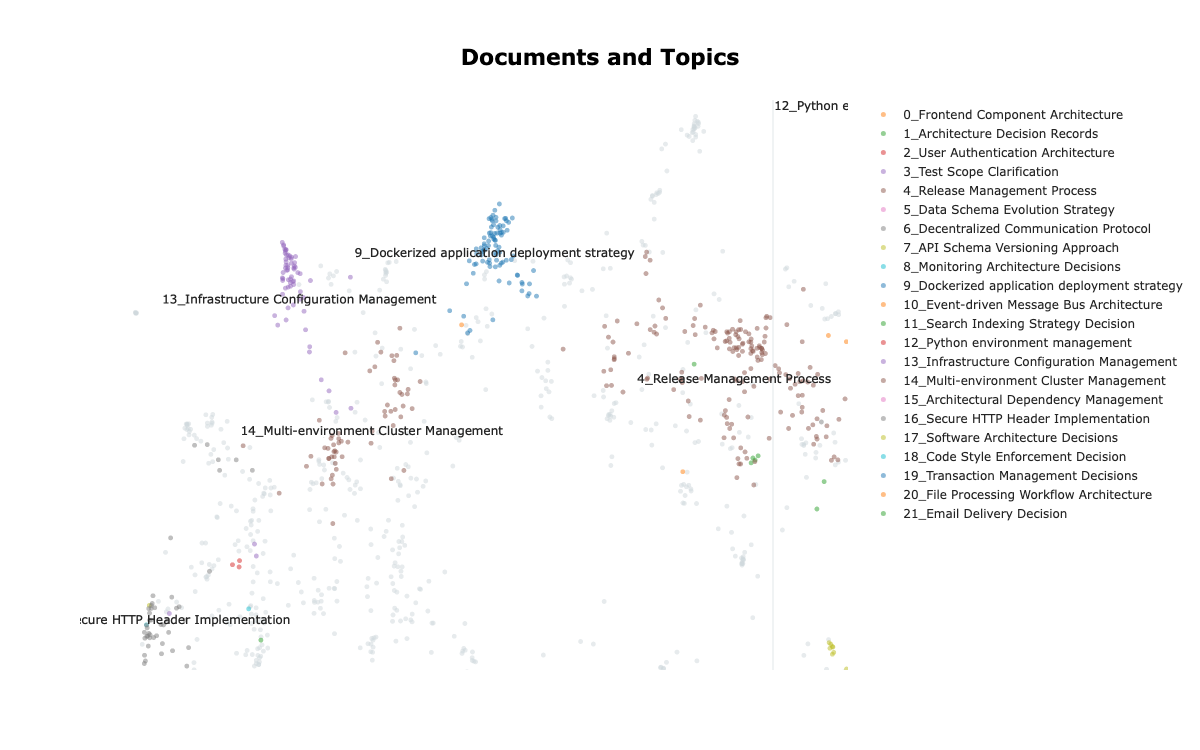
\includegraphics[scale=0.5]{figures/BerTopic_Original/zoomed_docs_infra.jpeg}
            \caption{ADRs related to cloud and infrastructure are located  closer in the embedding space}
            \label{fig:infra_docs}
        \end{figure}
        
        Examining the topics from a different perspective, a similarity matrix can be created to determine how clearly the topics have been separated by the model. This can also provide insights into the quality of the labels derived from the LLM, as conceptually similar topics should have a high similarity score and vise versa. The results are presented in figure \ref{fig:similarity_matrix_orginal}. 
        
        \begin{figure}[h]
            \centering
            \hspace*{-2cm} 
            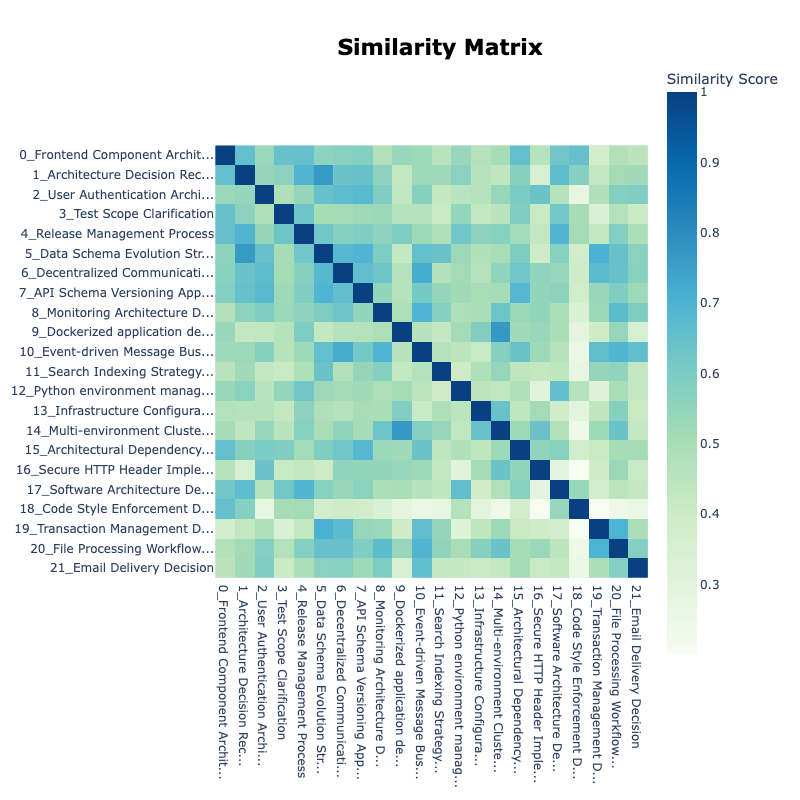
\includegraphics[scale=0.55]{figures/BerTopic_Original/heatmap_original.png}
            \caption{ADR topic similarity matrix}
            \label{fig:similarity_matrix_orginal}
        \end{figure}
        
        Following the previous patterns, some topics appear to be clearly separated and others intertwined. For example, decisions about database transaction management and data schema evolution have a high similarity score of 0.7, whereas architectural decisions about containerization and code style formats present a lower score of 0.28. An observation can be made, from the color distribution and scale in the matrix, that many topic pairs, including irrelevant ones, have relatively high similarity, with the lowest being close to 0.2. The lowest score is related to code styling formats topic and the secure HTTP header implementation document cluster while the highest, approaching 0.77 is compares dockerized application architectural decisions with decisions related to kubernetes cluster management. The high correlation, may be attributed to the similarity of the general theme of ADRs, with it being software architecture.

        To enhance the clarity of the results and create larger, more information-rich clusters, outlier reduction was applied to the topics, ensuring that only semantically similar documents were assigned to each cluster following the initial analysis. By utilizing the pre-calculated probabilities of an unlabeled document's likelihood of belonging to a specific cluster, the number of outliers was reduced to 704. The similarity threshold was set at 10\%, meaning outlier ADRs were included in the nearest topic cluster as long as they shared at least 10\% similarity. This low similarity threshold was chosen to maximize the number of documents assigned to a topic while isolating true outliers for further examination . The updated topic and document graph can be seen in figure \ref{fig:docs_reduced}.
        
        % \begin{figure}[ht]
        %     \centering
        %     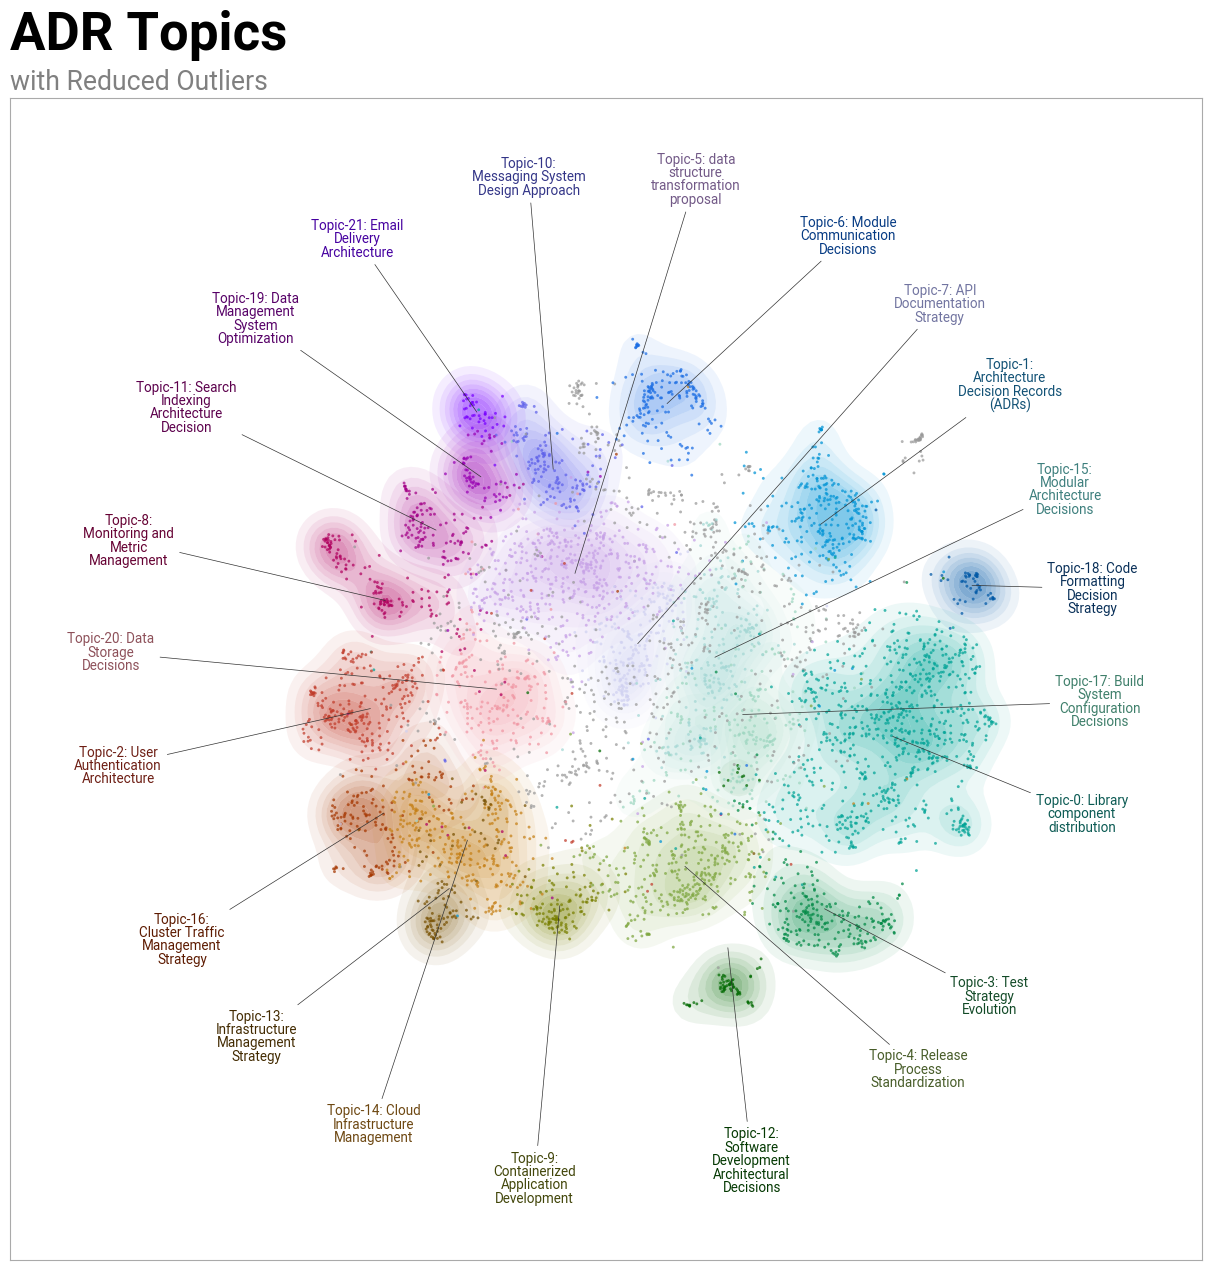
\includegraphics[scale=0.4]{figures/BerTopic_Reduced/datamap_reduced_outliers.png}
        %     \caption{Datamap of documents after outlier reduction}
        %     \label{fig:datamap_reduced}
        % \end{figure}
        
        Topics now cover larger areas in the embedding space and there is more topic coverage in the center parts of the axes. Topic clusters have been extended to include ADRs with more distance, modifying their initial state. From a visual perspective, clusters do not appear overly altered although outliers have been reduced by 72\% which indicates promising results. The remaining outliers are also more apparent, indicated in grey data points and will be used for later analysis to determine the reason for their low similarity.

        \begin{figure}[h]
            \centering
            \hspace*{-2.2cm} 
            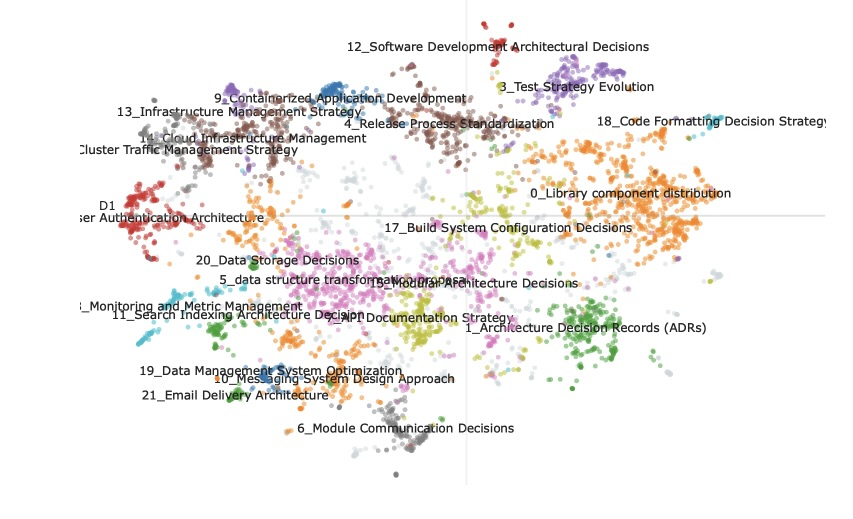
\includegraphics[scale=0.65]{figures/BerTopic_Reduced/docs_reduced_outliers.jpeg}
            \caption{Document embedding representation after outlier reduction}
            \label{fig:docs_reduced}
        \end{figure}

        In regards to topic similarity, the newly introduced documents, increased cluster diversity, indicated by the lowered similarity scores across all pairs of topics in figure \ref{fig:similarity_matrix_reduced}. Semantically similar pairs also retained their higher score while irrelevant pair scores were reduced significantly, with the minimum being 0.02 between testing strategy decisions and library code component management,  indicating clearer topic separation. 

        \begin{figure}[h]
            \centering
            \hspace*{-2cm} 
            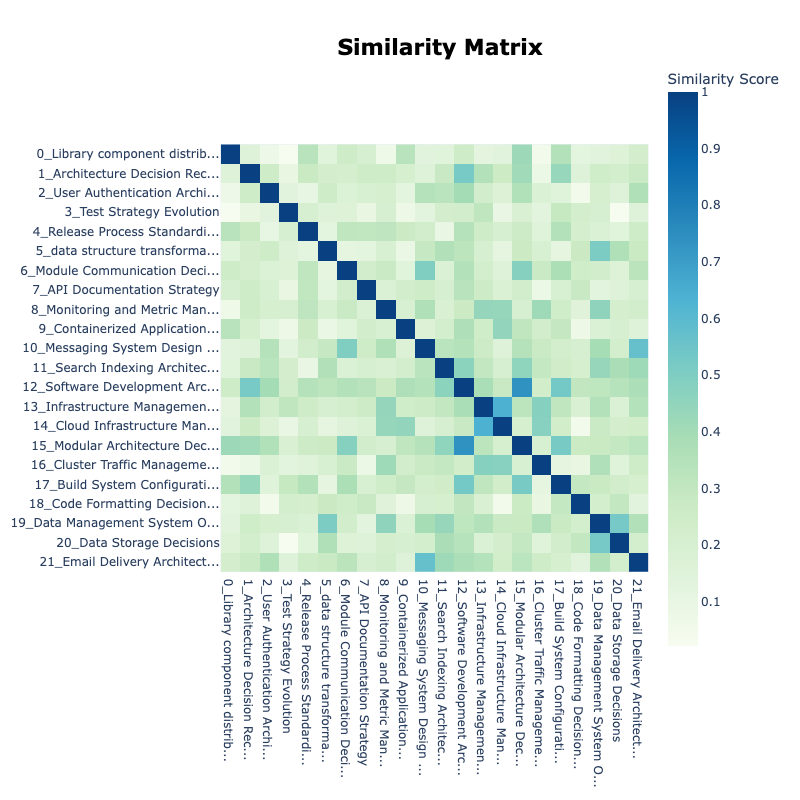
\includegraphics[scale=0.55]{figures/BerTopic_Reduced/similarity_matrix_reduced_outliers.png}
            \caption{ADR topic similarity matrix with reduced outliers}
            \label{fig:similarity_matrix_reduced}
        \end{figure}

        All research questions were answered using the results after the outlier reduction due to improved clarity. RQ3 also considered only the 704 final outliers as the filtering ensured their high degree of dissimilarity. A complete representation of the defined topics can be found in table 6.1.
        After closer examination of keywords and representative documents, three topics have been manually renamed from the original LLM representation. Topic ``Library component distribution'' has been renamed to ``Frontend Component and Design Decisions'' and ``Software Development Architectural Decisions'' has been changed to ``Python Development Decisions'' in line with its keyword representation. The later, was modified drastically due to the LLM prompt explicitly mentioning not to use names of specific technologies. Lastly, ``Module Communication Decisions'' was renamed to ``Distributed Systems Communication Decisions'' due to the vast majority of documents referring to distributed system decisions such as blockchain node communication.
        
        \begin{longtable}{|m{5cm}|c|c|c|c|c|c|}
    \hline
    % Nygard , Tyree \& Akerman , Alexandrian Pattern, Business Case, MADR , Planguage
    \textbf{Feature} & \textbf{NY} & \textbf{TA} & \textbf{AP} & \textbf{BC} & \textbf{MD} & \textbf{PL} \\
    \hline
    \textbf{Title} & + & + & - & + & + & + \\
    \hline
    \textbf{Status} & + & + & - & + & + & + \\
    \hline
    \textbf{Context/Background} & + & - & + & + & + & + \\
    \hline
    \textbf{Problem/Issue} & + & + & + & + & + & + \\
    \hline
    \textbf{Forces/Decision Drivers} & - & - & + & - & + & - \\
    \hline
    \textbf{Decision} & + & + & + & + & + & + \\
    \hline
    \textbf{Options} & - & - & - & + & + & + \\
    \hline
    \textbf{Solution} & + & + & + & + & + & + \\
    \hline
    \textbf{Consequences
    /Implications} & + & + & + & + & + & + \\
    \hline
    \textbf{Motivation/
    Rationale} & - & + & - & - & + & + \\
    \hline
    \textbf{Assumptions} & - & + & - & - & - & - \\
    \hline
    \textbf{Related Decisions} & - & + & - & - & - & - \\
    \hline
    \textbf{Stakeholders} & - & - & - & - & - & + \\
    \hline
    \textbf{Pros and Cons} & - & - & - & - & + & - \\
    \hline
    \caption{Comparison of ADR Templates}
    \label{table:adr_template_comparison}
\end{longtable}

    \section{RQ1: What are the most frequently discussed software architecture topics in ADRs?}

        To determine which topics are more prevalent in our dataset, the total number of ADRs per topic were counted and sorted. Then, for each topic, its document count was expressed as a\%age of total ADRs in the data. The results are presented in the bar chart in figure \ref{fig:docs_per_topic_percentage}. We will take a look at some notable ones. At a first glance, topics seem to be evenly distributed. The most frequent topic by a large margin, totaling 14.34\% of all documents is represented by the title ``Front-end Component Architecture'', its most frequent keywords are ``react'', ``component'', ``typescript'', ``npm'', ``framework'', ``frontend'', ``dependency'', ``design'', ``development'', ``angular''. This is the large orange cluster in figure \ref{fig:docs_reduced} that contains 770 ADRs. The second most frequent topic is labeled ``Data transformation proposal'' and its keywords are ``database'', ``schema'', ``sql'', ``metadata'', ``implementation'', ``data'', ``information'', ``structure'', ``migration'', ``json'' and seems to describe data related decisions such as storage and database structure. Other interesting topics include the topic labeled ``User Authentication Architecture'' that brings up security related topics at a 4,61\%, described by keywords as ``access control'', ``authorization'',``oauth'', ``authentication'',``openid'', ``access token'',``security'' and the topic named ``Cloud Infrastructure Management'' with ``kubernetes'', at a 5.4\% with ``cloud platform'', ``cluster'',``elasticsearch'', ``docker'',``pod'',``aws'', as dominan words. An ADR topic about architectural decisions and ADR themselves seems to emerge as the 5th most frequent topic containing 5.14\% of total documents. From its keywords, ``architectural record'', ``documentation'', ``changelog'', ``record architecture'', ``document'', ``structure'' it seems to also revolve around documentation and probably represents some of the first ADRs in each repository that state the need for ADRs and their usage moving forward. From the file cleaning process, at least 35 of those ADRs were identified. Lastly, the least frequent topics are related to email monitoring and notifications and code formatting conventions as indicated by their titles ``Code Formatting Decision Strategy'' and ``Email Delivery Architecture'' at percentages of 0.8 and 0.93 respectively. 

        \begin{figure}[H]
            % \centering
            \hspace*{-3cm} 
            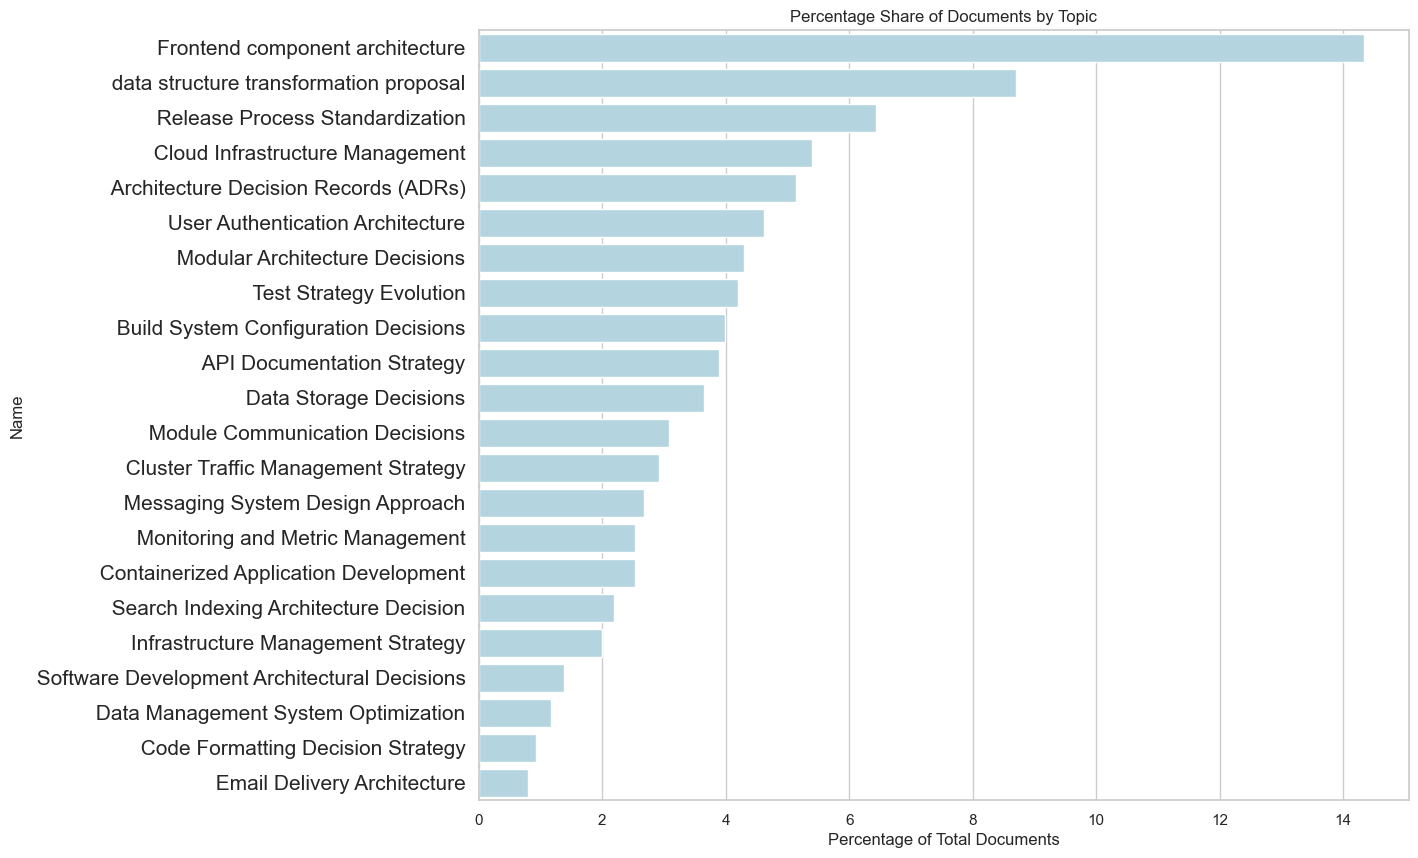
\includegraphics[scale=0.55]{figures/percentage_topics.png}
            \caption{Documents per topic as a percentage of total documents}
            \label{fig:docs_per_topic_percentage}
        \end{figure}

        % todo: include tree sort 

    \section{RQ2: How many topics from the general software architecture space are present in the ADRs?}

        Before determining which subset of topics from ADRs exist in the software architecture landscape, we must define a set of broad categories that architects have to consider when making design decisions. This is not a trivial task, as many trends, styles and general topics are implicit and documentation about actual architectural practices and decisions is limited.\cite{arch_patterns_in_practice_TOPICS}. In addition, design decisions can also be made to satisfy system attributes. Prominent attributes include availability, usability, performance, security, testability, modifiability and usability which are not topics but more so, systemic qualities that satisfy implied system or business needs \cite{patters+quality_requirements+tactics}.
        
        Architectural patterns, on the other hand, refer to a set of pre-defined styles and techniques for solving common reoccurring architectural problems, are more tangible but system-specific. \cite{Patterns+ArchDecisions}. Some popular patterns are Layers, Pipes-Filters, Model View Controller (MVC), Broker and Client–Server and are derived from the component-connector conceptual model \cite{survey_arch_patterns}. These aspects of decisions alone, do not constitute valid categorizations for our analysis as they refer to concepts that are either too implementation-specific or too broad. 
        
        Combining the two, we get architectural tactics. Architectural tactics ``serve as the
        meeting point between the quality attributes and the software architecture`` \cite{patters+quality_requirements+tactics}. Tactics are essentially specific measures taken to improve the quality attributes of the system. For example, an architect may decide to incorporate authentication and authorization into a system which in turn enhances security. Or referring to the findings of the previous question, a project may decide to use a specific frontend development framework in order to promote reusability if the framework allows for reusable code components. A comprehensive collection of tactics to satisfy specific system quality attributes, can be found in the Software Architecture in Practice book \cite{software_arch_in_practice_book}. 
        
        To answer RQ2, each topic identified from the previous question's results was examined and interpreted based on its frequent keywords and LLM representation, aiming to match it with any specific architectural pattern, tactic, or technique that fulfills a particular quality attribute. If the associated quality attributes are not immediately clear, a deeper dive into the topic was necessary, reviewing its representative ADRs, and attempting to identify several potential quality attributes, as we can't conclusively determine the true intents of each ADR author. This is an empirical approximation since many ADRs mentioned the potential adoption of very specific technologies and tools rather than architectural patterns and architectures of system components, which is not ideal when trying to examine architectural styles used. Furthermore, many topics refer to sub-processes and conceptually lower level techniques and some patterns were identifiable in subsets of the topic's documents.
        
        Future research could try to increase the total number of topics and closely examine each cluster to uncover additional patterns that may be overshadowed by more prominent ones within the cluster. This approach was not used as more clusters produced less comprehensive topics of ADRs and the sample size of each topic decreased by several orders of magnitude. The results of the comparison are presented in table \ref{table:topic_tactic}. Two semantically similar topics have been merged into larger categories, namely ``data management'' and ``cloud infrastructure'', reducing the total number of considered topics to 20.

        % { \small
%         \begin{longtable}{|p{3.8cm}|p{3cm}|p{2.2cm}|p{2.57cm}|p{2.8cm}|}
%         \caption{Topic Tactic Analysis}
%         \label{table:topic_tactic}
%         \hline
%         \textbf{Topic} & \textbf{Tactic} & \textbf{Pattern} & \textbf{Style} & \textbf{Quality Attribute} \\
%         \hline
%         \endfirsthead
    
%         \hline
%         \textbf{Topic} & \textbf{Tactic} & \textbf{Pattern} & \textbf{Style} & \textbf{Quality Attribute} \\
%         \hline
%         \endhead
        
%         \hline
%         \endfoot
        
%         \hline
%         \endlastfoot
        
%         Frontend Component and Design Decisions & Modularization & Component-Based & N/A & Reusability, Modifiability \\
%         \hline
%         Architecture Decision Records (ADRs) & Documentation & N/A & N/A & Maintainability \\
%         \hline
%         User Authentication Architecture & Authentication and Authorization & N/A & N/A & Security \\
%         \hline
%         Test Strategy Evolution & Automated Testing & N/A & N/A & Testability, Modifiability \\
%         \hline
%         Release Process Standardization & Continuous Integration/Continuous Deployment (CI/CD) & N/A & N/A & Maintainability, Reliability \\
%         \hline
%         Database Schema Management and Data Management System Optimization & Database Normalization, Data Optimization & N/A & Data-Centric & Maintainability, Performance, Efficiency \\
%         \hline
%         Module Communication Decisions & Asynchronous Messaging & Publish-Subscribe & Event-Driven & Performance, Scalability \\
%         \hline
%         API Documentation and Design Strategy & API Documentation & RESTful API & Representational State Transfer (REST) & Interoperability, Usability \\
%         \hline
%         Monitoring and Metric Management & Monitoring and Logging & N/A & N/A & Reliability, Maintainability \\
%         \hline
%         Containerized and Cloud Infrastructure Management & Containerization, Container Orchestration & Microservices & Service-Oriented Architecture (SOA) & Scalability, Availability, Modifiability \\
%         \hline
%         Messaging System Design Approach & Event-Driven Messaging & Event-Driven & N/A & Performance, Scalability \\
%         \hline
%         Search Indexing Architecture Decision & Indexing & N/A & N/A & Performance, Efficiency \\
%         \hline
%         Python Development Decisions & Scripting & N/A & N/A & Maintainability, Flexibility \\
%         \hline
%         Infrastructure Management Strategy & Infrastructure as Code & N/A & N/A & Scalability, Efficiency \\
%         \hline
%         Modular Architecture Decisions & Modularization & Modular Architecture & N/A & Modifiability, Reusability \\
%         \hline
%         Cluster Traffic and Load Management & Load Balancing & N/A & N/A & Performance, Availability \\
%         \hline
%         Build System Configuration Decisions & Configuration Management & N/A & N/A & Maintainability, Reliability \\
%         \hline
%         Code Formatting Decision Strategy & Code Quality & N/A & N/A & Maintainability, Readability \\
%         \hline
%         Data Storage Decisions & Data Storage Management & N/A & N/A & Performance, Data Integrity \\
%         \hline
%         Email Delivery Architecture & Notification Management & N/A & N/A & Usability, Reliability \\
%         \hline
%         \end{longtable}
%     }



{\small
    \begin{longtable}{|p{5cm}|p{6cm}|p{3cm}|}
        \caption{Topic Tactic Analysis}
        \label{table:topic_tactic}
        \hline
        \textbf{Topic} & \textbf{Tactic/Pattern/Style} & \textbf{Quality Attribute} \\
        \hline
        \endfirsthead
        
        \hline
        \textbf{Topic} & \textbf{Tactic/Pattern/Style} & \textbf{Quality Attribute} \\
        \hline
        \endhead
        
        \hline
        \endfoot
        
        \hline
        \endlastfoot
        
        Frontend Component and Design Decisions & Modularization, Component-Based, Model-View-Controller (MVC) & Reusability, Modifiability) \\
        \hline
        Architecture Decision Records (ADRs) & Documentation & Maintainability \\
        \hline
        User Authentication Architecture & Authentication and Authorization & Security \\
        \hline
        Test Strategy Evolution & Automated Testing & Testability, Modifiability \\
        \hline
        Release Process Standardization & Continuous Integration/Continuous Deployment (CI/CD) & Maintainability, Reliability \\
        \hline
        Database Schema Management and Data Management System Optimization & Pipes and Filters, Big Data Architecture, Database Normalization & Maintainability, Performance, Efficiency \\
        \hline
        Distributed Systems Communication Decisions & Peer-to-Peer, Distributed Architecture & Security, Reliability \\
        \hline
        API Documentation and Design Strategy & API Documentation, Client-Server, Representational State Transfer (REST) & Interoperability, Usability \\
        \hline
        Monitoring and Metric Management & Monitoring and Logging & Reliability, Maintainability \\
        \hline
        Containerized and Cloud Infrastructure Management & Containerization, Container Orchestration, Microservices, Service-Oriented Architecture (SOA), Cloud Computing Architecture & Scalability, Availability, Modifiability \\
        \hline
        Messaging System Design Approach & Event-Driven, Broker Model & Performance, Scalability \\
        \hline
        Search Indexing Architecture Decision & Indexing & Performance, Efficiency \\
        \hline
        Python Development Decisions & Scripting & Maintainability, Flexibility \\
        \hline
        Infrastructure Management Strategy & Infrastructure as Code & Scalability, Efficiency \\
        \hline
        Modular Architecture Decisions & Model-View-Controller (MVC), Modularization, Modular Architecture & Modifiability, Reusability \\
        \hline
        Cluster Traffic and Load Management & Load Balancing, Cloud Computing Architecture & Performance, Availability \\
        \hline
        Build System Configuration Decisions & Configuration Management & Maintainability, Reliability \\
        \hline
        Code Formatting Decision Strategy & Code Quality & Maintainability, Readability \\
        \hline
        Email Delivery Architecture & Client-Server, Notification Management & Usability, Reliability \\
        \hline
    \end{longtable}
}

        Overall, many of the most popular tactics, styles and patterns are present in the data indicating that open source projects mostly adhere to the same architecture principles. The diversity of architectural topics is also notable. Factoring in the percentage share of each topic relative to the tactic used, the Model-View-Controller (MVC) model is widely used, with many ADRs also referencing cloud computing topics and patterns. This confirms the findings from a recent study on trends in software architecture.\footnote{https://www.oreilly.com/radar/the-topics-to-watch-in-software-architecture/} Additionally, other well-established patterns such as Microservices, RESTful API, and Service-Oriented Architecture (SOA) are represented. The same study, conducted at the O’Reilly Software Architecture Conference in 2019, a year before our dataset was extracted, highlighted significant topics including microservices, testing, data, and monitoring, which matches our findings. On the opposite side, many ADRs, heavily focused on web development decisions which saw a heavy decline in topic trend. Notable missing topics include AI and machine learning, as well as a broader coverage of security practices and patterns such as the Layered Pattern, Blackboard, and Monolithic applications.
        
    \section{RQ3: Which ADR topics cannot be classified, and what are the reasons behind this?}
        From the main analysis, 707 ADRs could not be classified to a specific topic so they remained outliers. This could have been a result of several factors. Firstly, the minimum cluster size was initially set to 40 documents, meaning that topics present in less than 40 ADRs were considered outliers due to their limited presence in the dataset. Furthermore, outlier ADRs could refer to very specific project or technology decisions, which could disrupt the representations of larger clusters, making them more challenging to analyze semantically. As a result, these ADRs were excluded.
        
        For the outlier analysis, ADRs that were not assigned to topics were isolated and further topic modelling was performed on them to uncover their themes. This time, the numbers of documents per cluster was lowered to 10 aiming to uncover niche, underrepresented topics in the main dataset. Since the LLM could not produce satisfactory representations, topics were identified based on their frequent keywords in the respective ADRs. The results are presented in figure \ref{fig:outlier_datamap}.
        
        ADRs were clustered into 17 evenly distributed topics comprising of 20-80 documents. Most clusters are clearly separated in the embedding space. Outliers seem to focus on more implementation-specific topics such as api designs as indicated by topic 9, referring to GraphQL, tools such as hosting platforms seen in topic 12 referring to Heroku, and other decisions about project tactics and techniques such as caching (topic 8), tenancy (topic 4) and payment handling (topic 2). Environment variable management, time handling and routing (topics 14, 5 and 13) are also notable topics that concerned architects but to a lesser degree. In summary, the ADRs remained unclassified due to their small number in the main dataset rather than their abstract nature. They represent valid topics and strategies in software engineering, indicating that they could be integrated into the main topics if the dataset were expanded with more documents.
        
        \begin{figure}[H]
            \centering
            \hspace*{-1.2cm} 
            \includegraphics[scale=0.55]{figures/outlier_datamap.png}
            \caption{Outlier Document Datamap}
            \label{fig:outlier_datamap}
        \end{figure}

    \newpage
    \section{Threats to Validity}
    This study, like any empirical research, faces several threats to validity that must be addressed. Firstly, the topic modelling approach relies heavily on its hyperparameters that can alter the results with each run. The hyperparameters chosen were deemed satisfactory after many trials and the assessment of quality of each run was subjective in nature \cite{subjective_topic_modelling}. In addition, preprocessing steps, although close to popular industry practices, relied on personal observation and choice when it comes to areas of word filtering. If excluded words were to be changed, the results may differ. Furthermore, the dataset consisted primarily of ADRs from open-source GitHub projects, which may not fully represent ADRs from proprietary or enterprise environments. Readers should exercise caution when extending these results to a broader context, especially considering the relatively small amounts of documents in the dataset. When it comes to topic representation, the use of LLMs for topic titles might not have captured the full semantic meaning of each ADR in each cluster, as only 4 of the ADRs were delivered as prompts to the model each time, along with the most frequent keywords. The prompt used to make the requests to the model was also a result of fine tuning and in the end, highly subjective. This could potentially lead to oversimplification or misclassification and exact topic titles could not be replicated due to the LLMs non-deterministic nature. Lastly, it needs to be considered that the ADRs analyzed in this study, derived from a snapshot of the state of GitHub, that is evolving on a daily basis. The repositories used can be modified or deleted at any time, just like we observed in the dataset scrapping process, hindering the reproducability of the results.

\chapter{Conclusions and Sustainability of ADRs} 

    \section{Summary of Findings}
        This thesis aimed to explore the role and effectiveness of Architectural Design Records (ADRs) in documenting architectural decisions within open source software repositories. It also examined the architectural decision process in software engineering and how ADRs fit into it's lifecycle. By performing numerous topic modelling techniques such as TF-IDF, LDA, and BERTopic, we analyzed and enriched a dataset of ADRs extracted from GitHub.
        With the help of LLMs, findings revealed a diverse range of topics within the documents, with an emphasis in areas such as frontend development, data management, user authentication, and cloud infrastructure management that concern architects and engineers alike, in line with the current industry trends. We were also able to identify popular tactics, topics and patterns from the general software architecture landscape such as microservices and containerization, application tenancy and API design that satisfy common quality attributes of systems. More niche topics also revealed decisions about payment handling, caching and adoption of specific technology tools and platforms. However, as adoption of ADRs remains limited, the study highlighted gaps in design topics related to object oriented design, data-centric app architecture and patterns such as the Layered approach and security related patterns.
    \section{Sustainability Practices}
        When it comes to sustainability, ADRs appear to be a valuable tool that assists the capturing of architectural knowledge, avoiding knowledge vaporization, ensuring consistent and informed decision-making, and facilitating maintenance and evolution of software systems. ADRs, due to their ease of use and lightweight nature, can also help contribute to better impact analysis, understanding of design rationale, and knowledge sharing across teams and stakeholders, all while creating a traceable chain of decisions. Sustainable practices for ADR usage, derived from common complaints of software architects via a plethora of studies, include maintaining a centralized repository for ADRs that acts as a source of truth, integrating ADRs into regular project workflows, and encouraging collaborative decision-making processes all while making these processes as frictionless and time consuming as possible. Organizations, drawing inspiration from experienced practitioners and companies in the industry, could also provide training and resources to promote the effective use of ADRs among their architects and developers. In general, ADRs is a straightforward way to transform the architectural knowledge acquired from the architecting process from implicit to explicit. They help convey the ``why'' of a decision, not the ``what'' and ``how'', in an efficient and easy-to-manage way. By embedding ADRs into the development lifecycle and using tools like version control, teams can ensure that ADRs remain current, accessible, and useful. 
    \section{Future Directions}
        Future research on ADRs can focus on several directions. Firstly, expanding the dataset to include ADRs from private and enterprise environments could provide further understanding of architectural decision-making practices across different contexts.
        
        Leveraging a larger dataset, machine learning models can be trained to assist architects when making architectural decisions, replacing outdated and inflexible tools. This can also be integrated with commonly used architectural knowledge management tools to produce, store, index and manage fully automated ADR knowledge bases across organizations. Autonomous agents can also be leveraged to monitor developer's code via pull requests to check whether it conforms with the architectural standards proposed in previous ADRs from the organizational knowledge base. This could reduce architectural drift and provide real time architectural guidelines in the development process. However, it is unclear how many ADRs will be needed to achieve this, as research on ADRs and artificial intelligence methods is limited. 
        
        ADRs could also be incorporated as a topic in evidence-based software engineering (EBSE) studies \cite{evidence_based_software_eng} to assess their impact on decision-making quantitative metrics. Finally, exploring the creation of dependency graphs from ADR back-links, that encompass the whole architectural decision chain, is also an option. This could potentially trace the status of a software project at any given point in time, preventing conflict, and ensuring composability across decisions and system components.

\bibliographystyle{plain}
\bibliography{references/ref-Intro}

\end{document}

